\clearpage
%\setcounter{page}{1}
% \maketitlesupplementary

\onecolumn

{
    \clearpage
    \centering
    \Large
    \textbf{\thetitle}\\
    \vspace{0.5em}Supplementary Material \\
    \vspace{1.0em}
}

This document reports additional material concerning ``Stereo Anywhere: Robust Zero-Shot Deep Stereo Matching Even Where Either Stereo or Mono Fail". Specifically:

\begin{itemize}
    \item First, we present an extended description of our proposed architecture in \cref{sec:method}, including detailed formulations of the monocular correlation volume (\cref{subsec:mono_corr}), differentiable monocular scaling (\cref{subsec:diff_mono}), cost volume augmentation (\cref{subsec:cost_aug}), volume truncation (\cref{subsec:vol_trunc}), and training supervision (\cref{subsec:training}). 

    \item We then report extensive ablation studies in \cref{sec:ablation} demonstrating how our stereo matching architecture effectively generalizes across different state-of-the-art monocular depth networks (\cref{subsec:ablation_VFM}), showing consistent improvements over baseline stereo methods regardless of the specific VFM employed. 
    Then, we show qualitatively the impact of the truncated cost volume augmentation on disparity estimation on non-Lambertian surfaces (\cref{subsec:vol_trunc_qual}). Furthermore, we include an analysis of runtime performance and memory consumption (\cref{subsec:runtime}) across different input resolutions and VFMs.  

    \item Finally, we present extensive qualitative results in \cref{subsec:qual} across multiple datasets, demonstrating the effectiveness of our method in dealing with challenging scenarios such as non-Lambertian surfaces, transparent objects and textureless regions.
\end{itemize}

\section{Method Overview: Additional Details}

In this section, we enrich the description of \method architecture.

\subsection{Monocular Correlation Volume}
\label{subsec:mono_corr}

Given the monocular depth estimations $\textbf{M}_L \in \mathbb{R}^{1 \times H \times W}$ and $\textbf{M}_R \in \mathbb{R}^{1 \times H \times W}$, we aim to estimate the normal maps $\nabla_L \in \mathbb{R}^{3 \times \frac{H}{4} \times \frac{W}{4}}$ and $\nabla_R \in \mathbb{R}^{3 \times \frac{H}{4} \times \frac{W}{4}}$ to construct the 3D correlation volume $\mathbf{V}_M \in \mathbb{R}^{\frac{H}{4} \times \frac{W}{4} \times \frac{W}{4}}$.
We decide to use $\nabla_L$ and $\nabla_R$ instead of extracting additional features from $\textbf{M}_L$ and $\textbf{M}_R$ because $\textbf{M}_L$ and $\textbf{M}_R$ already provide high-level information.
Furthermore, normal maps can handle depth inconsistencies between $\textbf{M}_L$ and $\textbf{M}_R$ that can occur for example when a foreground object is visible only in a single view.
We downsample $\textbf{M}_L$ and $\textbf{M}_R$ to 1/4  -- bilinear interpolation, then we estimate $\nabla_L$ and $\nabla_R$  -- spatial gradient:

\small\begin{equation}
    \nabla = \frac{\nabla^*}{\lVert \nabla^* \rVert}, \quad \nabla^* = \begin{bmatrix}
        -\frac{\partial \left(\lambda\mathbf{M}_\frac{1}{4}\right)}{\partial x} & -\frac{\partial \left(\lambda\mathbf{M}_\frac{1}{4}\right)}{\partial y} & 1 \\
    \end{bmatrix}, \quad \lambda = \frac{1}{10}\cdot\frac{W}{4}
    \label{eq:normal_estimation}
\end{equation}\normalsize
where $\lambda$ is a gain factor that is proportional to $W$, which permits to achieve scale-invariant normal maps.

Given the absence of texture in normal maps, $\textbf{V}_M$ will be not ambiguous only in edges.
To alleviate this problem, we segment $\textbf{V}_M$  -- the relative depth priors from $\textbf{M}_L$ and $\textbf{M}_R$: doing so we aim to reduce the ambiguity by forcing the matching only in similar depth regions (\eg, foreground objects cannot match with background object since the correlation score is masked to zero).
Considering \cref{eq:vol_masking}, we calculate masks ${\mathcal{M}_L}^n$ and ${\mathcal{M}_R}^n$ as follows:

\small\begin{equation}
    ({\mathcal{M}_L}^n)_{ij} = \begin{cases}
        1\ \text{if}\ \frac{n}{N} \leq (\mathbf{M}_L)_{ij} < \frac{n+1}{N}\\
        0\ \text{otherwise}
    \end{cases} \quad ({\mathcal{M}_R}^n)_{ik} = \begin{cases}
        1\ \text{if}\ \frac{n}{N} \leq (\mathbf{M}_R)_{ik} < \frac{n+1}{N}\\
        0\ \text{otherwise}
    \end{cases}
    \label{eq:mask}
\end{equation}\normalsize

To further deal with the ambiguity, we improve the 3D Convolutional Regularization model $\phi_A$  -- an adapted version of CoEx \cite{bangunharcana2021correlate} correlation volume excitation that exploits both views $\textbf{M}_L$, $\textbf{M}_R$:

\small\begin{equation}
    ({\mathbf{V'}^s}_M)_{fijk} = \sigma\left(({{\mathbf{f}_L}^s})_{fij}\right) \odot \sigma\left(({{\mathbf{f}_R}^s})_{fik}\right) \odot ({\mathbf{V}^s}_M)_{fijk}
    \label{eq:our_coex}
\end{equation}\normalsize
where ${\mathbf{V'}^s}_M$ is the excited volume, $\sigma(\cdot)$ is the sigmoid function, $\odot$ is the element-wise product, ${\mathbf{V}^s}_M \in \mathbb{R}^{F \times \frac{H}{s} \times \frac{W}{s} \times \frac{W}{s}}$ is an intermediate correlation feature volume at scale $s$ with $F$ features inside module $\phi_A$,  ${\mathbf{f}_L}^s \in \mathbb{R}^{F \times \frac{H}{s} \times \frac{W}{s} \times 1}$ and ${\mathbf{f}_R}^s \in \mathbb{R}^{F \times \frac{H}{s} \times 1 \times \frac{W}{s}}$ are shallow 2D conv-features extracted from $\mathbf{M}_L$ and $\mathbf{M}_R$ downsampled at proper scale.

\subsection{Differentiable Monocular Scaling}
\label{subsec:diff_mono}

As detailed in \cref{subsec:corr_pyramids}, volume $\mathbf{V}^D_M$ is used also to estimate the coarse disparity maps $\hat{\mathbf{D}}_L$ $\hat{\mathbf{D}}_R$, while volume $\mathbf{V}^C_M$ is utilized to estimate confidence maps $\hat{\mathbf{C}}_L$ $\hat{\mathbf{C}}_R$.
$\hat{\mathbf{D}}_L$ $\hat{\mathbf{C}}_L$ and $\hat{\mathbf{D}}_R$ $\hat{\mathbf{C}}_R$ are used to scale respectively $\mathbf{M}_L$ and $\mathbf{M}_R$.
As described in \cref{eq:softmax_left}, we can estimate left disparity from a correlation volume  -- a softargmax operation on the last W dimension of $\mathbf{V}^D_M$ and  -- the relationship between left disparity and correlation.
Here we report an extended version of \cref{eq:softmax_left} with the explicit formula for softargmax operator:

\small\begin{equation} 
    (\hat{\mathbf{D}}_L)_{ij} = j - \left(\text{softargmax}_L (\mathbf{V}^D_M )\right)_{ij} = j - \sum_{d}^{\frac{W}{4}} d \cdot \frac{e^{(\mathbf{V}^D_M)_{ijd}}}{\sum_{f}^{\frac{W}{4}} e^{(\mathbf{V}^D_M)_{ijf}}}
    \label{eq:softmax_left2}
\end{equation}\normalsize

At the same time, given the relationship between right disparity and correlation $d_R=k_L-k_R$ we can estimate the right disparity performing a softargmax on the first $W$ dimension of $\mathbf{V}^D_M$:
\small\begin{equation}
    (\hat{\mathbf{D}}_R)_{ik} = \left(\text{softargmax}_R(\mathbf{V}^D_M)\right)_{ik} - k = \sum_{d}^{\frac{W}{4}} d \cdot \frac{e^{(\mathbf{V}^D_M)_{idk}}}{\sum_{f}^{\frac{W}{4}} e^{(\mathbf{V}^D_M)_{ifk}}} - k
    \label{eq:softmax_right}
\end{equation}\normalsize

Disparity maps $\hat{\mathbf{D}}_L$ $\hat{\mathbf{D}}_R$ are used in combination with confidence maps $\hat{\mathbf{C}}_L$ $\hat{\mathbf{C}}_R$ to obtain a robust scaling.
We present an expanded version of the information entropy based confidence estimation (\cref{eq:confidence_left}), with the explicit formula for softmax operator:

\small\begin{equation}
    (\hat{\mathbf{C}}_L)_{ij} = 1  + \frac{\sum_{d}^{\frac{W}{4}} \left(\text{softmax}_L(\mathbf{V}_M^C)\right)_{ijd} \cdot \log_2 \left( \left(\text{softmax}_L(\mathbf{V}_M^C)\right)_{ijd} \right)}{\log_2(\frac{W}{4})} = 1  + \frac{\sum_{d}^{\frac{W}{4}} \frac{e^{(\mathbf{V}^C_M)_{ijd}}}{\sum_{f}^{\frac{W}{4}} e^{(\mathbf{V}^C_M)_{ijf}}} \cdot \log_2 \left( \frac{e^{(\mathbf{V}^C_M)_{ijd}}}{\sum_{f}^{\frac{W}{4}} e^{(\mathbf{V}^C_M)_{ijf}}} \right)}{\log_2(\frac{W}{4})}
    \label{eq:confidence_left2}
\end{equation}\normalsize

In the same way, we estimate right confidence map $\hat{\mathbf{C}}_R$ performing a softmax operation on the first $W$ dimension of $\mathbf{V}^C_M$:

\small\begin{equation}
    (\hat{\mathbf{C}}_R)_{ik} = 1  + \frac{\sum_{d}^{\frac{W}{4}} \left(\text{softmax}_R(\mathbf{V}_M^C)\right)_{idk} \cdot \log_2 \left( \left(\text{softmax}_R(\mathbf{V}_M^C)\right)_{idk} \right)}{\log_2(\frac{W}{4})} = 1 + \frac{\sum_{d}^{\frac{W}{4}} \frac{e^{(\mathbf{V}^C_M)_{idk}}}{\sum_{f}^{\frac{W}{4}} e^{(\mathbf{V}^C_M)_{ifk}}} \cdot \log_2 \left( \frac{e^{(\mathbf{V}^C_M)_{idk}}}{\sum_{f}^{\frac{W}{4}} e^{(\mathbf{V}^C_M)_{ifk}}} \right)}{\log_2(\frac{W}{4})}
    \label{eq:confidence_right}
\end{equation}\normalsize


To improve the robustness of the scaling, we introduce a softLRC operator to classify occlusions as low-confidence pixels and consequentially mask out them from $\hat{\mathbf{C}}_L$ and $\hat{\mathbf{C}}_R$.
We define the softLRC operator as follows:

\small\begin{equation}
    \text{softLRC}_L(\mathbf{D},\mathbf{D}_R) = \frac{\log\left(1+\exp\left(T_\text{LRC}-\left| \mathbf{D}_L - \mathcal{W}_L(\mathbf{D}_L,\mathbf{D}_R) \right|\right)\right)}{\log(1+\exp(T_\text{LRC}))}
    \label{eq:softlrc}
\end{equation}\normalsize
where $T_\text{LRC}=1$ is the LRC threshold and $\mathcal{W}_L(\mathbf{D}_L,\mathbf{D}_R)$ is the warping operator that uses the left disparity $\mathbf{D}_L$ to warp the right disparity $\mathbf{D}_R$ into the left view. 

Finally, we can estimate the scale $\hat{s}$ and shift $\hat{t}$  -- a differentiable weighted least-square approach. We report here the expanded form of \cref{eq:scale_shift}:
\small\begin{equation}
    \min_{\hat{s}, \hat{t}} \left\lVert \sqrt{\hat{\mathbf{C}}_L}\odot\left[\left(\hat{s}\mathbf{M}_L + \hat{t}\right)  - \hat{\mathbf{D}}_L \right] \right\rVert_F + \left\lVert \sqrt{\hat{\mathbf{C}}_R}\odot\left[\left(\hat{s}\mathbf{M}_R + \hat{t}\right)  - \hat{\mathbf{D}}_R \right] \right\rVert_F 
    \label{eq:scale_shift2}
\end{equation}\normalsize
where $\lVert\cdot\rVert_F$ denotes the Frobenius norm.

\subsection{Cost Volume Augmentations}
\label{subsec:cost_aug}

Volume augmentations are necessary when the training set -- \eg, Sceneflow \cite{mayer2016large} -- does not model particularly complex scenarios where a VFM could be useful, for example, when experiencing non-Lambertian surfaces.
Without any augmentation of this kind, the stereo network would simply overlook the additional information from the monocular branch.
As detailed in the main paper, we propose three volume augmentations and a monocular augmentation to overcome this issue.
In this supplementary section, we explain the rationale behind the introduction of each augmentation:

\begin{itemize}
    \item \textit{Volume Rolling}: non-Lambertian surfaces such as mirrors and glasses violate the geometry constraints, leading to a high matching peak in a wrong disparity bin. This augmentation emulates this behavior by shifting some among the matching peaks to a random position: consequentially, \method learns to retrieve the correct peak from the other branch. \\
    \item \textit{Volume Noising} and \textit{Volume Zeroing}: we introduce noise and false peaks into the correlation volume to simulate scenarios with texture-less regions, repeating patterns, and occlusions. \\
    \item \textit{Perfect Monocular Estimation}: instead of acting inside the correlation volumes, we can substitute the prediction of the VFM with a perfect monocular map  -- the ground truth normalized between $[0,1]$. This perfect prediction is noise-free and therefore the monocular branch of \method will likely gain importance during the training process.
\end{itemize}

\subsection{Volume Truncation}
\label{subsec:vol_trunc}

The proposed volume truncation strategy further helps \method to handle mirror surfaces.
Here we introduce additional details about fuzzy operators -- useful to make a boolean expression differentiable -- and the sigmoid curve used to truncate the volume $\mathbf{V}_S$  -- the truncate mask $(\mathbf{T})_{ij} = \left[\left((\hat{\mathbf{M}}_L)_{ij} >(\hat{\mathbf{D}}_L)_{ij}\right) \land (\mathbf{C}_M)_{ij} \right] \lor \left[ (\mathbf{C}_M)_{ij} \land \neg(\hat{\mathbf{C}}_L)_{ij} \right]$.

We can replace operators AND ($\land$), OR ($\lor$), NOT ($\neg$) and GREATER ($>$) inside $\mathbf{T}$ with the fuzzy counterparts $\text{AND}_\text{F}(A,B) = A \cdot B$, $\text{OR}_\text{F}(A,B) = A+B-A \cdot B$, $\text{NOT}_\text{F}(A) = 1- A$ and $\text{GREATER}_\text{F}(A,B) = \sigma(A-B)$, obtaining the fuzzy truncate mask $\mathbf{T}_\text{F}$:

\small\begin{equation}
    \begin{split}
        (\mathbf{T}_\text{F})_{ij} &= (\mathbf{T}^A_\text{F})_{ij} + (\mathbf{T}^B_\text{F})_{ij} - (\mathbf{T}^A_\text{F})_{ij} \cdot (\mathbf{T}^B_\text{F})_{ij}\\        
        (\mathbf{T}^A_\text{F})_{ij} &= (\mathbf{C}_M)_{ij} \cdot \sigma\left( (\hat{M}_L)_{ij} - (\hat{D}_L)_{ij} \right)\\
        (\mathbf{T}^B_\text{F})_{ij} &= (\mathbf{C}_M)_{ij} \cdot \left(1-(\hat{\mathbf{C}}_L)_{ij}\right)
    \end{split}
    \label{eq:truncate_mask_fuzzy}
\end{equation}\normalsize
where $\mathbf{T}^A_\text{F}$ and $\mathbf{T}^B_\text{F}$ are respectively the left section and the right section of the $\text{OR}_\text{F}$ of mask $\textbf{T}_\text{F}$.
Next, we can apply threshold $T_m$ to achieve the final fuzzy mask $\mathbf{T}'_\text{F}$ as follows:

\small\begin{equation}
    (\mathbf{T}'_\text{F})_{ij}=\sigma\left((\mathbf{T}_\text{F})_{ij}-T_m\right)
    \label{eq:truncate_mask_fuzzy_thresholded}
\end{equation}\normalsize.

Finally, we can use the fuzzy truncate mask $\mathbf{T}'_\text{F}$ and the scaled monocular map $\hat{\mathbf{M}_L}$ to generate the sigmoid-based truncation volume $\mathbf{V}_T$:

\small\begin{equation}
    (\mathbf{V}_T)_{ijk} = \left(1-(\mathbf{T}'_\text{F})_{ij}\right) + (\mathbf{T}'_\text{F})_{ij} \cdot \left[ \sigma\left(j - (\hat{\mathbf{M}}_L)_{ij} - k\right) \cdot (1-G) + G \right]
    \label{eq:truncate_vol}
\end{equation}\normalsize
where $G=0.9$ attenuates the impact of the truncation. 
The correlation volume $\mathbf{V}_S$ is truncated through an element-wise product with $\mathbf{V}_T$.

\subsection{Training Supervision}
\label{subsec:training}

We supervise the iterative module  -- the L1 loss with exponentially increasing weights \cite{lipson2021raft}:

\small\begin{equation}
    \mathcal{L}_\text{A} = \sum_{l=1}^L{\gamma^{L-l}\lVert \mathbf{D}^l-\mathbf{D}_\text{Lgt} \rVert_1}
    \label{eq:loss_raft}
\end{equation}\normalsize
where L is the total number of iterations made by the update operator and $\mathbf{D}_\text{Lgt}$ is the ground truth of the left disparity map.
Furthermore, we supervise the outputs $\hat{\mathbf{D}}_L$, $\hat{\mathbf{D}}_R$, $\hat{\mathbf{M}}_L$, $\hat{\mathbf{M}}_R$, $\hat{\mathbf{C}}_L$, $\hat{\mathbf{C}}_R$ of the monocular branch -- respectively L1 loss and normal loss for $\hat{\mathbf{D}}_L$ $\hat{\mathbf{D}}_R$, L1 loss for $\hat{\mathbf{M}}_L$ $\hat{\mathbf{M}}_R$ and Binary Cross Entropy (BCE) loss for $\hat{\mathbf{C}}_L$ $\hat{\mathbf{C}}_R$:

\small\begin{equation}
    \mathcal{L}_\text{B} = \lVert \hat{\mathbf{D}}_L - \mathbf{D}_\text{Lgt} \rVert_1 + \psi \left\lVert \mathbf{1} - \nabla_L\cdot\hat{\nabla}_L \right\rVert_1 \quad \left( \nabla_L\cdot\hat{\nabla}_L \right)_{ij} = \sum_h (\nabla_L)_{hij} \cdot (\hat{\nabla}_L)_{hij}
    \label{eq:loss_coarse_disp_left}
\end{equation}\normalsize
\small\begin{equation}
    \mathcal{L}_\text{C} = \lVert \hat{\mathbf{D}}_R - \mathbf{D}_\text{Rgt} \rVert_1 + \psi \left\lVert \mathbf{1} - \nabla_R\cdot\hat{\nabla}_R \right\rVert_1 \quad \left( \nabla_R\cdot\hat{\nabla}_R \right)_{ik} = \sum_h (\nabla_L)_{hik} \cdot (\hat{\nabla}_L)_{hik}
    \label{eq:loss_coarse_disp_right}
\end{equation}\normalsize
\small\begin{equation}
    \mathcal{L}_\text{D} = \lVert \hat{\mathbf{M}}_L - \mathbf{D}_\text{Lgt} \rVert_1  \quad \mathcal{L}_\text{E} = \lVert \hat{\mathbf{M}}_R - \mathbf{D}_\text{Rgt} \rVert_1 
    \label{eq:loss_scaled_disp}
\end{equation}\normalsize
\small\begin{equation}
    \mathcal{L}_\text{F} = \text{BCE}(\hat{\mathbf{C}}_L,\mathbf{C}_\text{Lgt}), \quad (\mathbf{C}_\text{Lgt})_{ij} = \frac{\log\left(1+\exp\left(T_\text{LRC}-\left| (\hat{\mathbf{D}}_L)_{ij} - (\mathbf{D}_\text{Lgt})_{ij}  \right|\right)\right)}{\log(1+\exp(T_\text{LRC}))}
    \label{eq:loss_coarse_conf_left}
\end{equation}\normalsize
\small\begin{equation}
    \mathcal{L}_\text{G} = \text{BCE}(\hat{\mathbf{C}}_R,\mathbf{C}_\text{Rgt}), \quad (\mathbf{C}_\text{Rgt})_{ik} = \frac{\log\left(1+\exp\left(T_\text{LRC}-\left| (\hat{\mathbf{D}}_R)_{ik} - (\mathbf{D}_\text{Rgt})_{ik}  \right|\right)\right)}{\log(1+\exp(T_\text{LRC}))}
    \label{eq:loss_coarse_conf_right}
\end{equation}\normalsize
where $\psi=10$ is the normal loss weight, $\mathbf{D}_\text{Rgt}$ is the ground truth of the right disparity map, $\hat{\nabla}_L$ $\hat{\nabla}_R$ are the normal maps estimated respectively from $\hat{\mathbf{D}}_L$ $\hat{\mathbf{D}}_R$, $\nabla_L\cdot\hat{\nabla}_L$ and $\nabla_R\cdot\hat{\nabla}_R$ are the dot product between normal maps, and $\mathbf{C}_\text{Lgt}$ $\mathbf{C}_\text{Rgt}$ are the confidence ground truth.
The final supervision loss $\mathcal{L}$ is the sum of all previous partial losses:
\small\begin{equation}
    \mathcal{L} = \mathcal{L}_A + \mathcal{L}_B + \mathcal{L}_C + \mathcal{L}_D + \mathcal{L}_E + \mathcal{L}_F + \mathcal{L}_G
    \label{eq:total_loss}
\end{equation}\normalsize

\section{Additional Ablation Studies}
\label{sec:ablation}
In this section, we report additional studies concerning the performance of \method.

\subsection{Generalization to Different VFMs}
\label{subsec:ablation_VFM}

In the main paper, we assumed Depth Anything v2 \cite{depth_anything_v2} as the VFM fueling \method, since it is the latest state-of-the-art model being published at the time of this submission. 
However, any VFM for monocular depth estimation would be suitable for this purpose, either current or future ones. To confirm this argument, we conducted some experiments by replacing Depth Anything v2 with other VFMs that appeared on arXiv in the last months, yet that are not been officially published. Among them, we select DepthPro \cite{depthpro}, MoGe \cite{wang2024moge} and Lotus \cite{he2024lotus}.

Table \ref{tab:morevfm2} shows the results achieved by \method variants -- different VFMs on Booster and LayeredFlow. We can appreciate how the different flavors of \method always outperform the baseline stereo model \cite{lipson2021raft}. In general, Depth Anything v2 remains the best choice to deal with non-Lambertian surfaces, with Moge allowing for small improvements on some metrics over the Booster dataset.



\begin{table*}[ht]
\centering
\renewcommand{\tabcolsep}{14pt}
\scalebox{0.78}{
\begin{tabular}{|l||rrrrr|rrrr|}
\multicolumn{1}{c}{} & \multicolumn{5}{c}{Booster (Q)} & \multicolumn{4}{c}{LayeredFlow (E)} \\
\hline
 \multirow{2}{*}{Model} & \multicolumn{4}{c}{Error Rate (\%)} & Avg. & \multicolumn{3}{c}{Error Rate (\%)} & Avg. \\
  & $>2$ & $>4$ & $>6$ & $>8$ & (px) & $>1$ & $>3$ & $>5$ &(px) \\
\hline\hline
{Baseline} \cite{lipson2021raft}
&  17.84 &  13.06 &  10.76 &  9.24 &  3.59
&  89.21 &  79.02 & 71.61 &  19.27 \\
{\method{}  -- DAv2 \cite{depth_anything_v2}}
& 9.96 & 5.81 & 4.48 & 3.79 & 1.36
& 80.83 & 58.21 & 46.48 & 12.14 \\
{\method{}  -- DepthPro \cite{depthpro}}
& 10.53 & 7.02 & 5.79 & 5.13 & 2.40
& 78.76 & 61.11 & 51.04 & 14.43 \\
{\method{}  -- MoGe \cite{wang2024moge}}
& 9.47 & 5.77 & 4.49 & 3.84 & 1.44
& 84.27 & 68.67 & 58.89 & 16.22 \\
{\method{}  -- Lotus \cite{he2024lotus}}
& 12.44 & 8.71 & 7.58 & 6.98 & 3.21
& 86.04 & 62.75 & 49.47 & 13.98 \\
\hline

\end{tabular}}\vspace{-0.2cm}
\caption{\textbf{Non-Lambertian Generalization of \method w.r.t VFMs.} We measure the impact of different monocular depth estimation networks. Networks trained on SceneFlow \cite{mayer2016large}.
}
\label{tab:morevfm2}
\end{table*}

Table \ref{tab:morevfm1} shows the results achieved by the different VFMs on the zero-shot generalization benchmark. Also in this case, we can appreciate how any \method variant yields comparable accuracy, with some VFMs like Moge yielding some improvements over Depth Anything v2 on ETH3D, KITTI 2012 and 2015 at the expense of lowering the accuracy on Middlebury 2014 and 2021. Interestingly, we can observe an important drop in accuracy by using DepthPro on Middlebury 2021, due to several failures by the model itself on the scenes of this dataset.


\begin{table*}[ht]
\centering
\renewcommand{\tabcolsep}{6pt}
\scalebox{0.62}{
\begin{tabular}{|l||rrrr|rrrr|rrrr|rrrr|rrrr|}
\multicolumn{1}{c}{} & \multicolumn{4}{c}{Middlebury 2014 (H)} & \multicolumn{4}{c}{Middlebury 2021} & \multicolumn{4}{c}{ETH3D} & \multicolumn{4}{c}{KITTI 2012} & \multicolumn{4}{c}{KITTI 2015} \\
\hline
 \multirow{2}{*}{Model} & \multicolumn{3}{c}{bad $>2$} & Avg. & \multicolumn{3}{c}{bad $>2$} & Avg. & \multicolumn{3}{c}{bad $>1$} & Avg. & \multicolumn{3}{c}{bad $>3$} & Avg. & \multicolumn{3}{c}{bad $>3$} & Avg. \\
  & All & Noc & Occ & (px) & All & Noc & Occ & (px) & All & Noc & Occ & (px) & All & Noc & Occ & (px) & All & Noc & Occ & (px) \\
\hline\hline
{Baseline} \cite{lipson2021raft} 
& 11.15 & 8.06 & 29.06 &  1.55 
& 12.05 & 9.38 & 37.89 & 1.81 
& 2.59 & 2.24 &  8.78 & 0.25 
&  4.80 &  3.70 &  28.54 &  0.89 
&  5.44 &  4.69 &  13.52 &  1.16 \\
\hline\hline
{\method{}  -- DAv2 \cite{depth_anything_v2}} 
& 7.07 & 4.76 & 20.77 & 0.97
& 8.38 &  5.86 & 32.87 & 1.10 
&  2.39 &  2.16 & 5.82 &  0.28 
& 3.94 & 3.03 & 21.02 & 0.85 
& 3.98 & 3.29 & 10.55 & 0.97 \\
{\method{}  -- DepthPro \cite{depthpro}} 
& 6.58 & 4.32 & 20.05 & 0.99 
& 15.13 & 12.52 & 41.16 & 8.97 
& 2.74 & 2.54 & 6.09 & 0.44 
& 3.13 & 2.25 & 18.25 & 0.75 
& 3.79 & 3.10 & 10.53 & 0.95 \\
{\method{}  -- MoGe \cite{wang2024moge}} 
& 7.79 & 5.23 & 22.86 & 1.21 
& 9.86 & 7.30 & 33.48 & 1.28 
& 1.28 & 1.09 & 3.78 & 0.21 
& 2.85 & 2.00 & 17.40 & 0.73 
& 3.22 & 2.57 & 8.97 & 0.89 \\
{\method{}  -- Lotus \cite{he2024lotus}} 
& 7.35 & 4.96 & 21.71 & 1.07 
& 9.62 & 7.01 & 34.92 & 1.29 
& 2.68 & 2.44 & 6.04 & 0.31 
& 4.54 & 3.58 & 22.71 & 0.92 
& 3.88 & 3.21 & 10.36 & 0.95 \\

\hline
\end{tabular}}\vspace{-0.2cm}
\caption{\textbf{Generalization of \method w.r.t VFMs.} We measure the impact of different monocular depth estimation networks. Networks trained on SceneFlow \cite{mayer2016large}.
}
\label{tab:morevfm1}
\end{table*}


Finally, Figure \ref{fig:multiple_vfms} shows qualitative results obtained by the different variants of \method, highlighting only minor differences among the different predictions.

\begin{figure*}[h]
    \centering 
    \renewcommand{\tabcolsep}{1pt}
    \begin{tabular}{cccccc}

    \multirow{2}{*}{\small RGB} & \multirow{2}{*}{\small RAFT-Stereo \cite{lipson2021raft}} & \small \method & \small \method & \small \method & \small \method \\

     &  & \small -- DAv2 \cite{depth_anything_v2} & \small -- DepthPro \cite{depthpro} & \small -- MoGe \cite{wang2024moge} & \small -- Lotus \cite{he2024lotus} \\

    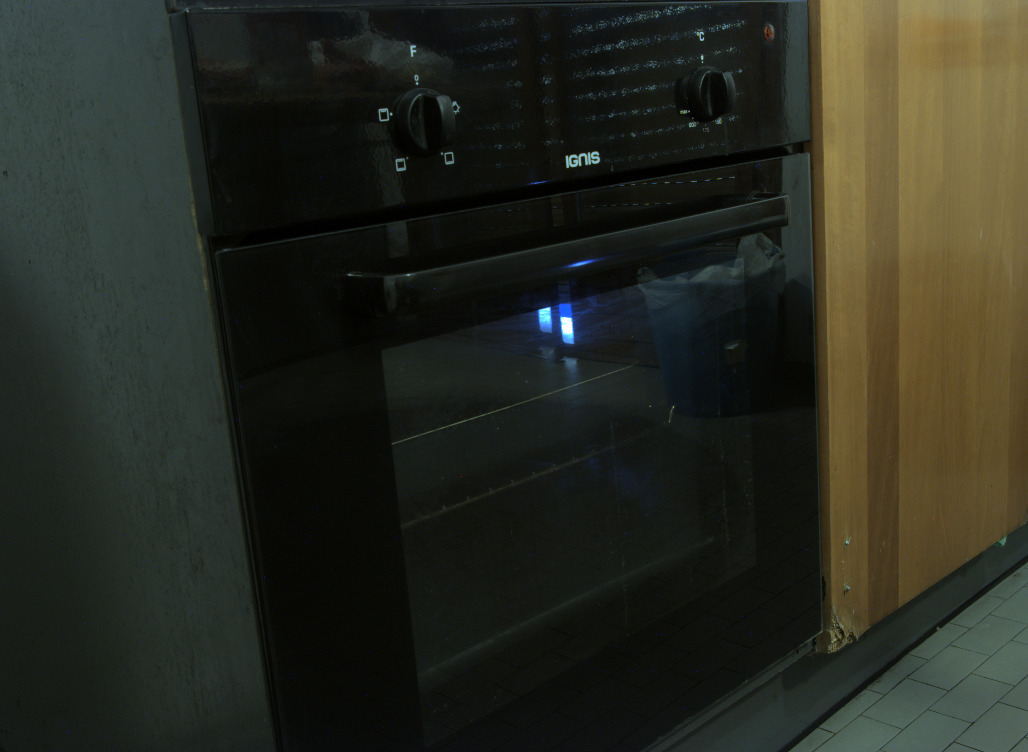
\includegraphics[width=0.16\linewidth]{imgs/multiple_vfms/booster_multiple_vfms/0.jpg} & 
    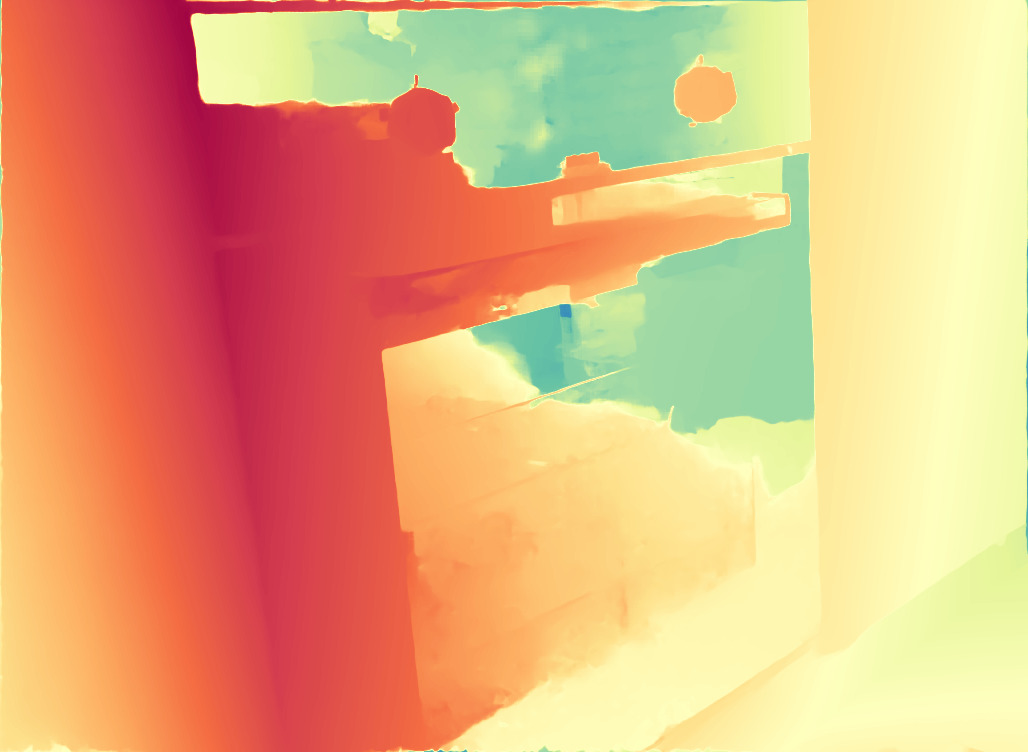
\includegraphics[width=0.16\linewidth]{imgs/multiple_vfms/booster_multiple_vfms/_raft-stereo.jpg} & 
    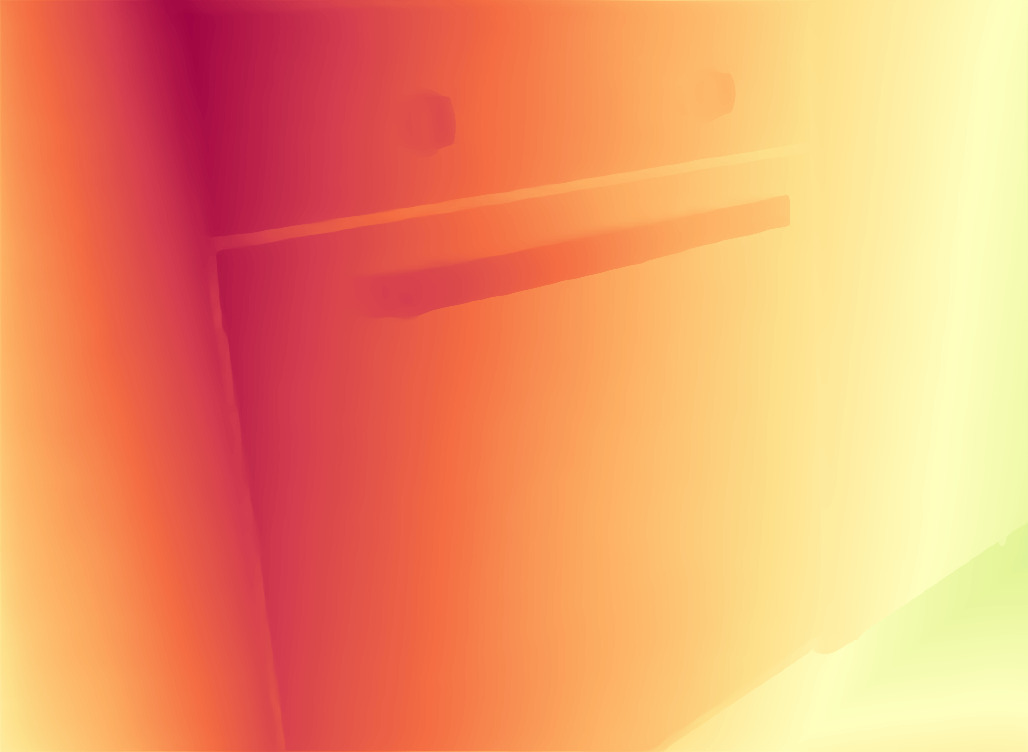
\includegraphics[width=0.16\linewidth]{imgs/multiple_vfms/booster_multiple_vfms/_ours_dav2.jpg} & 
    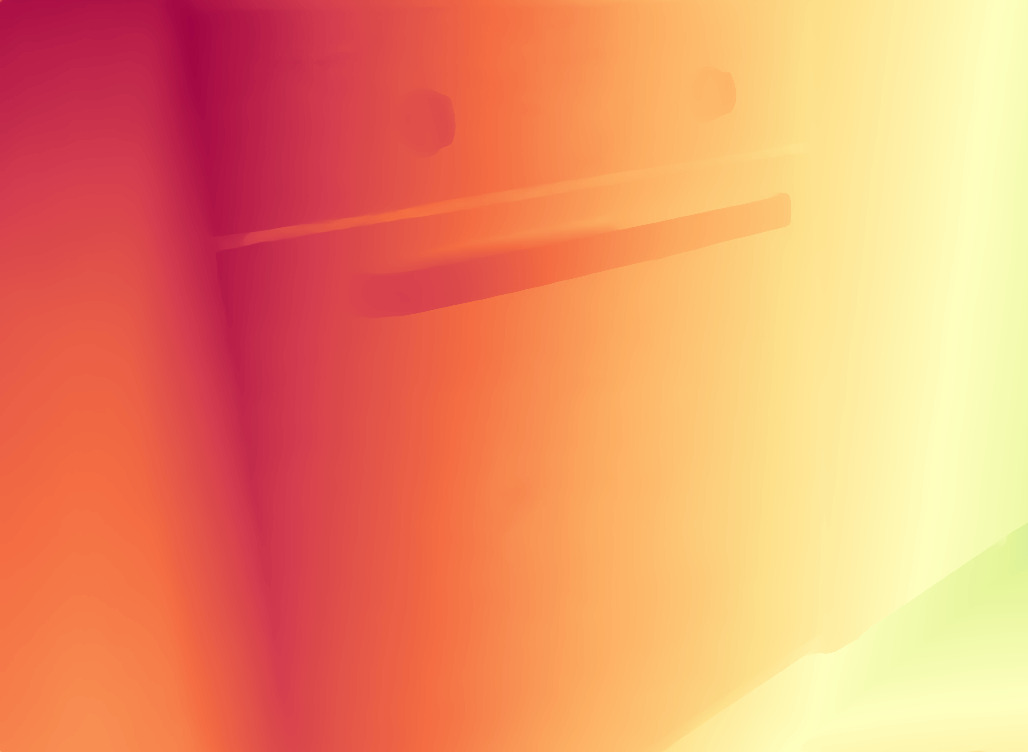
\includegraphics[width=0.16\linewidth]{imgs/multiple_vfms/booster_multiple_vfms/_ours_depthpro.jpg} & 
    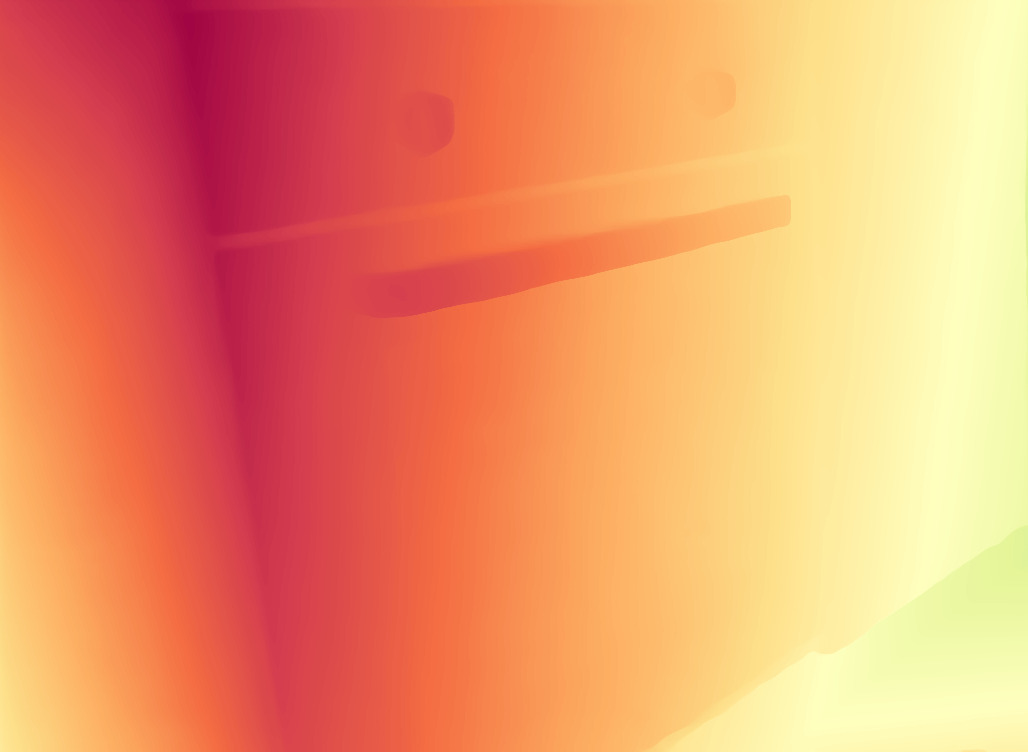
\includegraphics[width=0.16\linewidth]{imgs/multiple_vfms/booster_multiple_vfms/_ours_moge.jpg} & 
    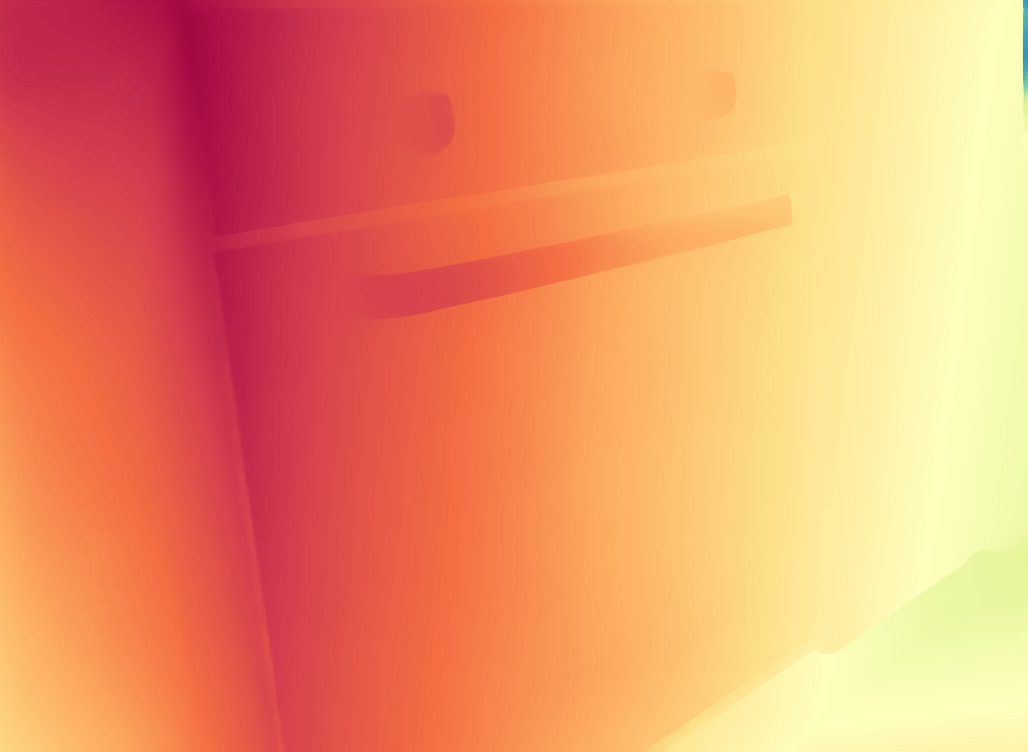
\includegraphics[width=0.16\linewidth]{imgs/multiple_vfms/booster_multiple_vfms/_ours_lotus.jpg} \\ 

    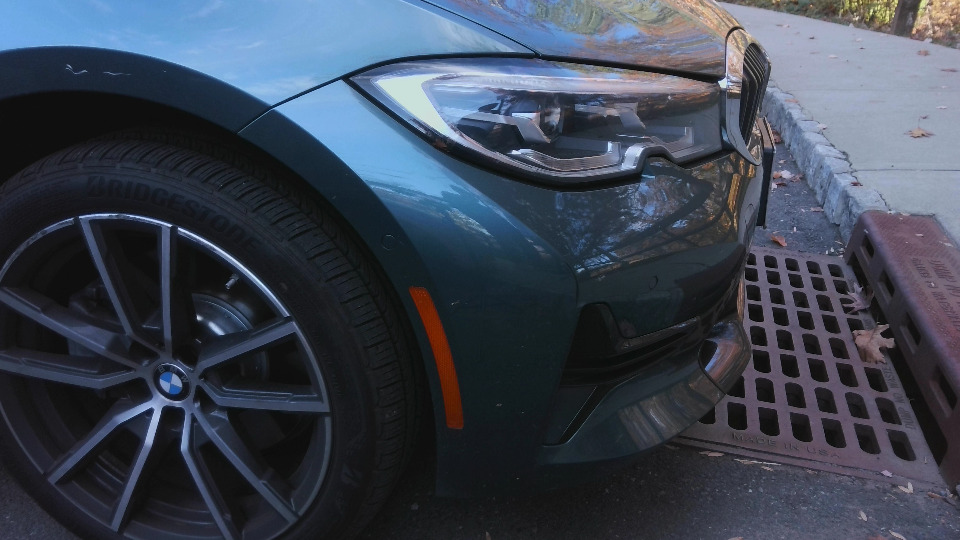
\includegraphics[width=0.16\linewidth]{imgs/multiple_vfms/layered/337.jpg} &
    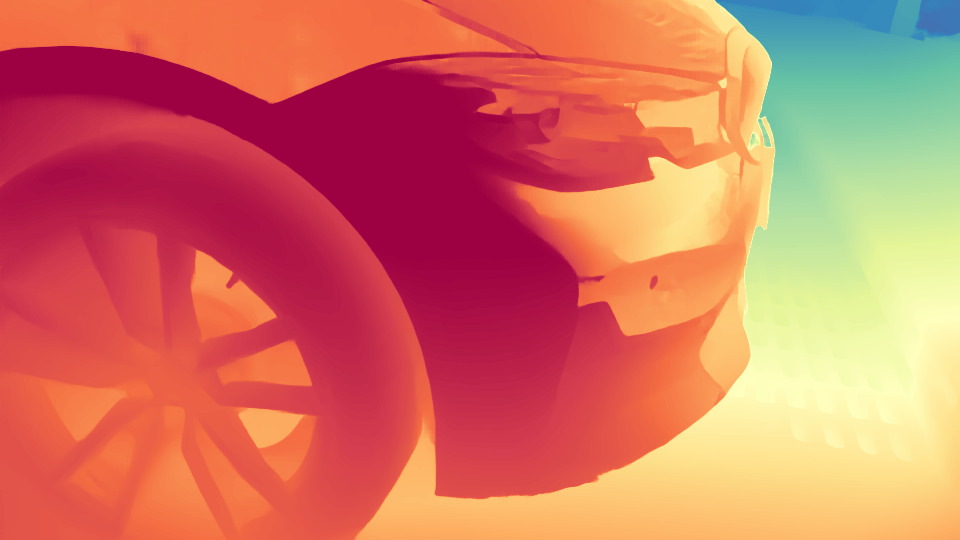
\includegraphics[width=0.16\linewidth]{imgs/multiple_vfms/layered/337_raft.jpg} &
    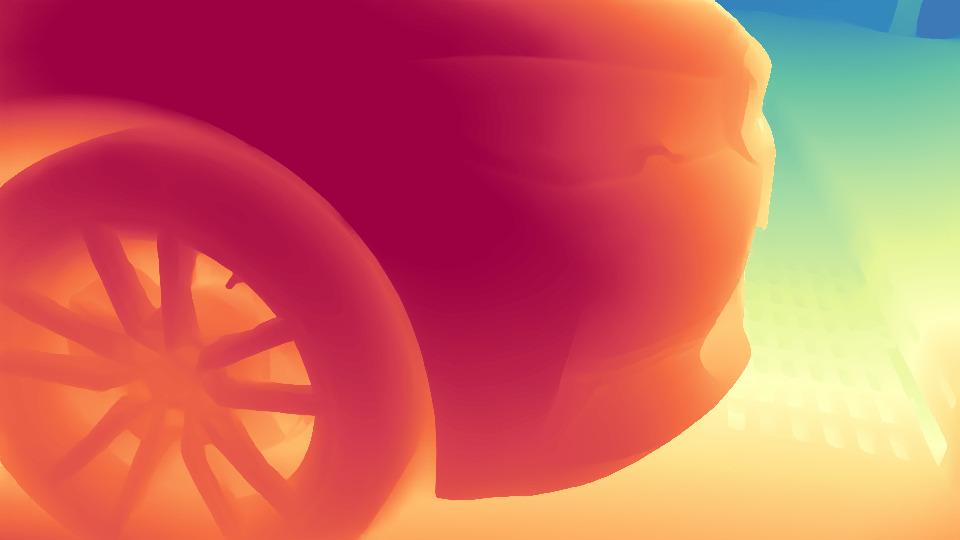
\includegraphics[width=0.16\linewidth]{imgs/multiple_vfms/layered/337_dav2.jpg} &
    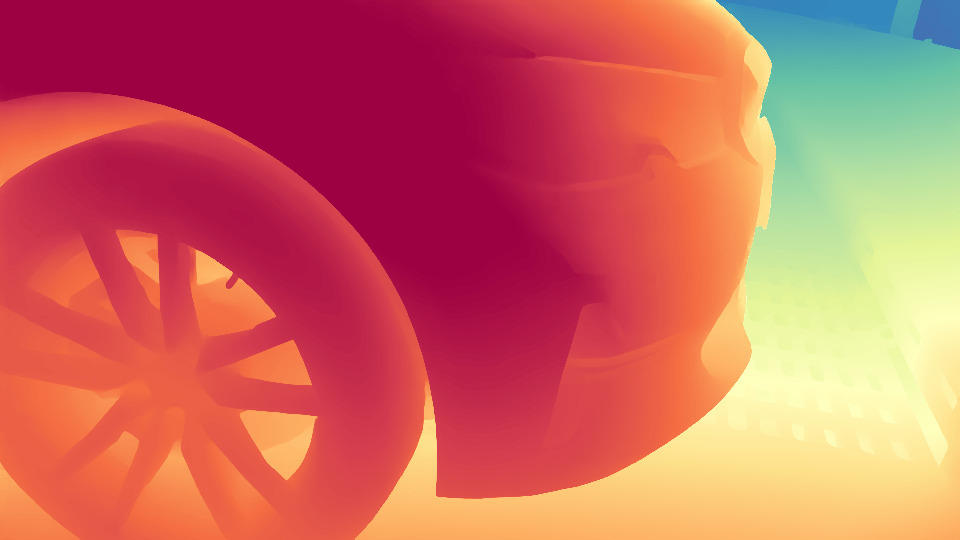
\includegraphics[width=0.16\linewidth]{imgs/multiple_vfms/layered/337_depthpro.jpg} &
    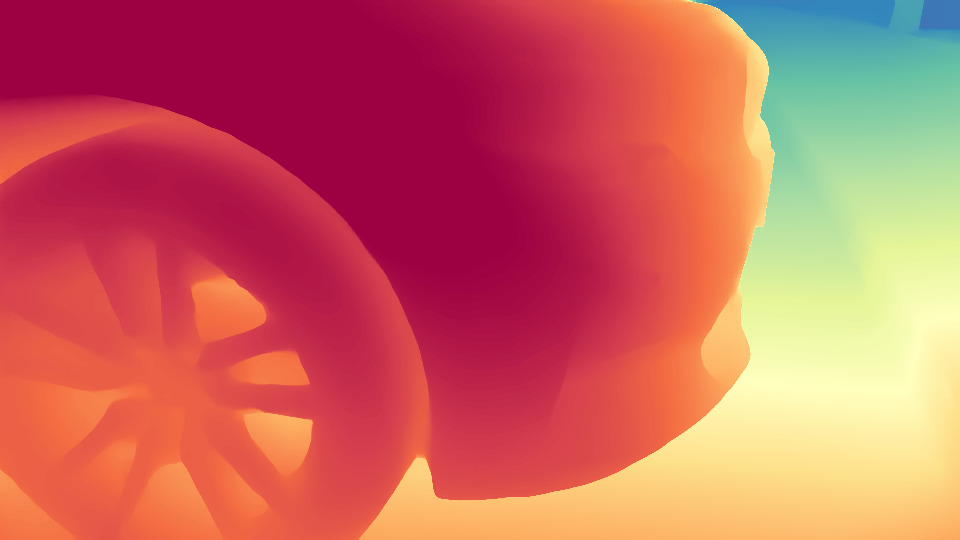
\includegraphics[width=0.16\linewidth]{imgs/multiple_vfms/layered/337_moge.jpg} &
    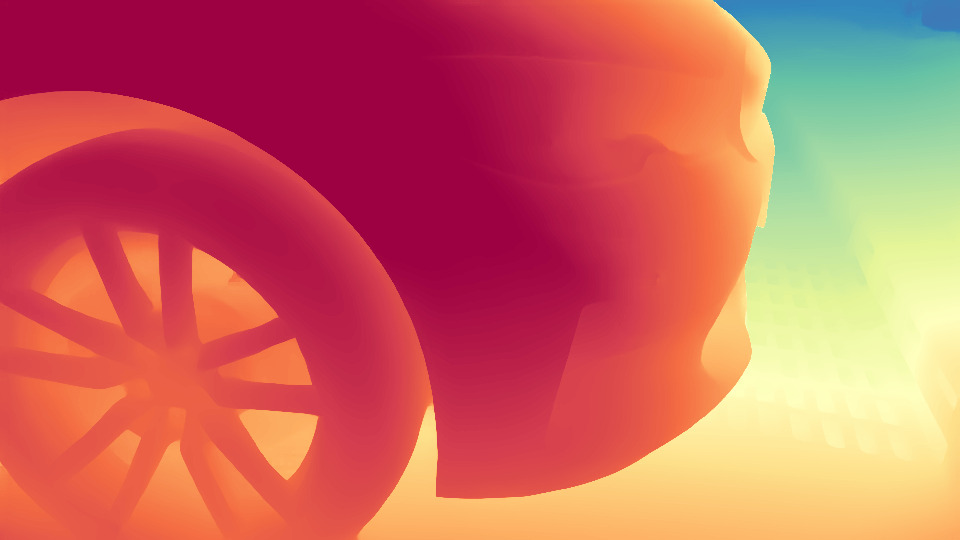
\includegraphics[width=0.16\linewidth]{imgs/multiple_vfms/layered/337_lotus.jpg} \\
    
    \end{tabular}\vspace{-0.3cm}
    \caption{\textbf{Qualitative Results -- Booster and LayeredFlow.} Predictions by RAFT-Stereo and \method{} -- different VFMs.}
    \label{fig:multiple_vfms}\vspace{-0.3cm}
\end{figure*}

\subsection{Impact of Cost Volume Truncation}
\label{subsec:vol_trunc_qual}

Cost volume truncation is a specific augmentation we apply to improve the results in the presence of mirrors. Figure \ref{fig:truncation} shows a qualitative example of predictions by \method (using Depth Anything v2) obtained by either not applying or by applying such augmentation. 
While \method alone cannot entirely restore the surface of the mirror starting from the priors provided by the VFM, applying cost volume truncation allows for predicting a much smoother and consistent surface.

\begin{figure*}[h]
    \centering 
    \renewcommand{\tabcolsep}{1pt}
    \begin{tabular}{ccc}

    \multirow{2}{*}{\small RGB} & \small \method & \small \method \\
    & \small w/o volume truncation & \small w/ volume truncation \\
    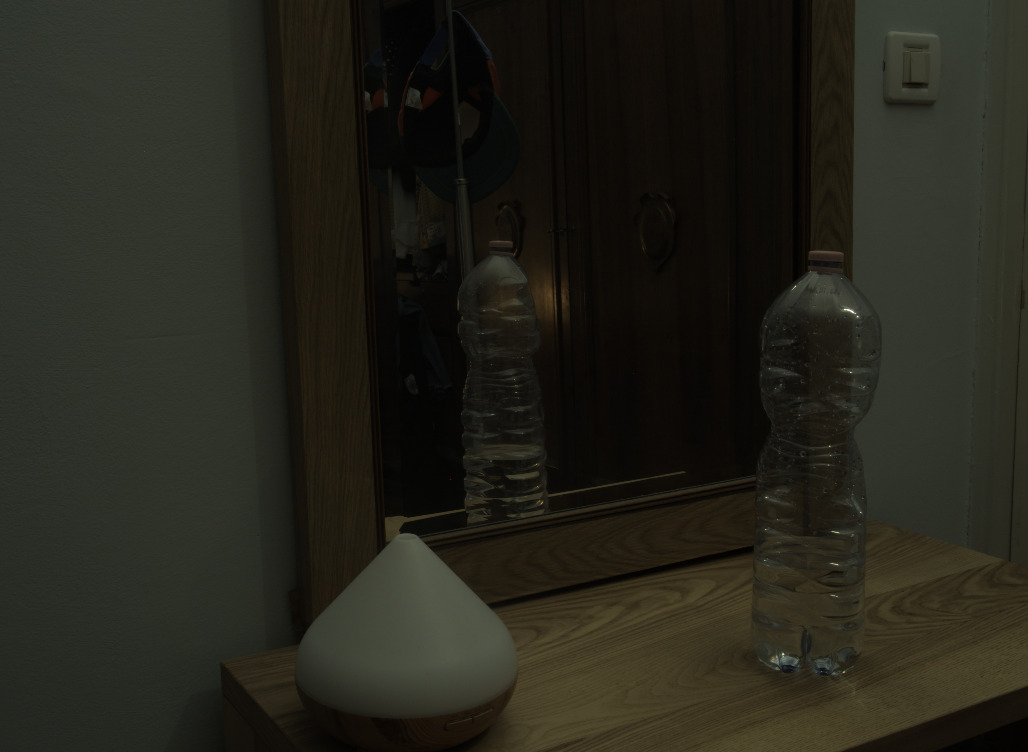
\includegraphics[width=0.3\linewidth]{imgs/booster/rgb/19.jpg} &
    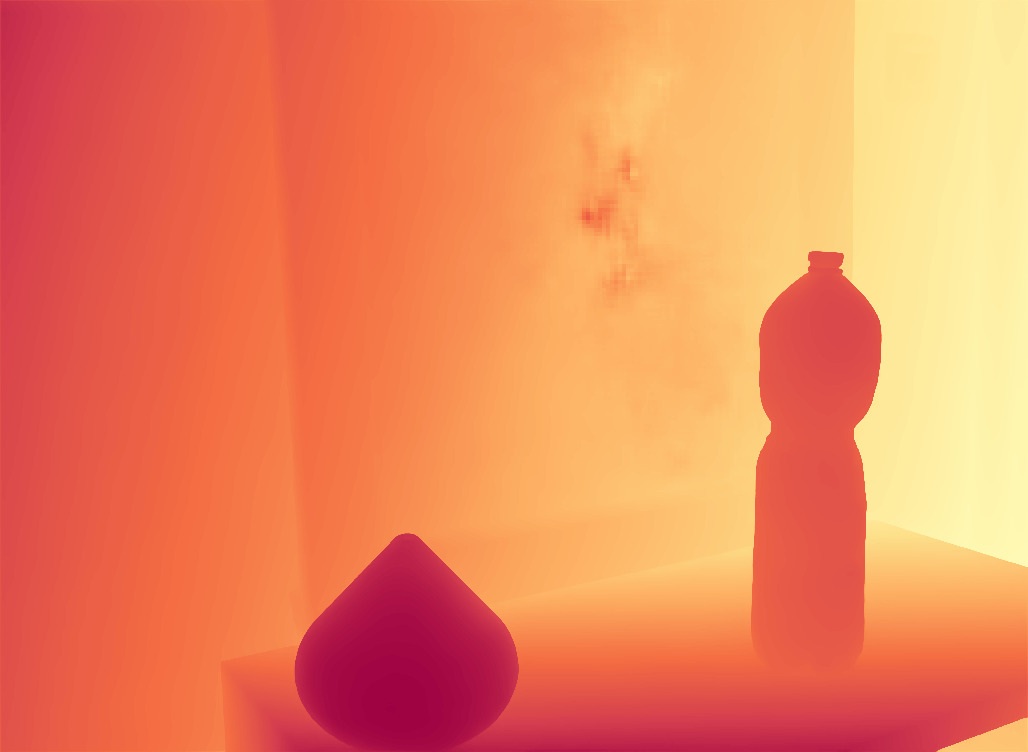
\includegraphics[width=0.3\linewidth]{imgs/mirror_without_truncation.jpg} &
    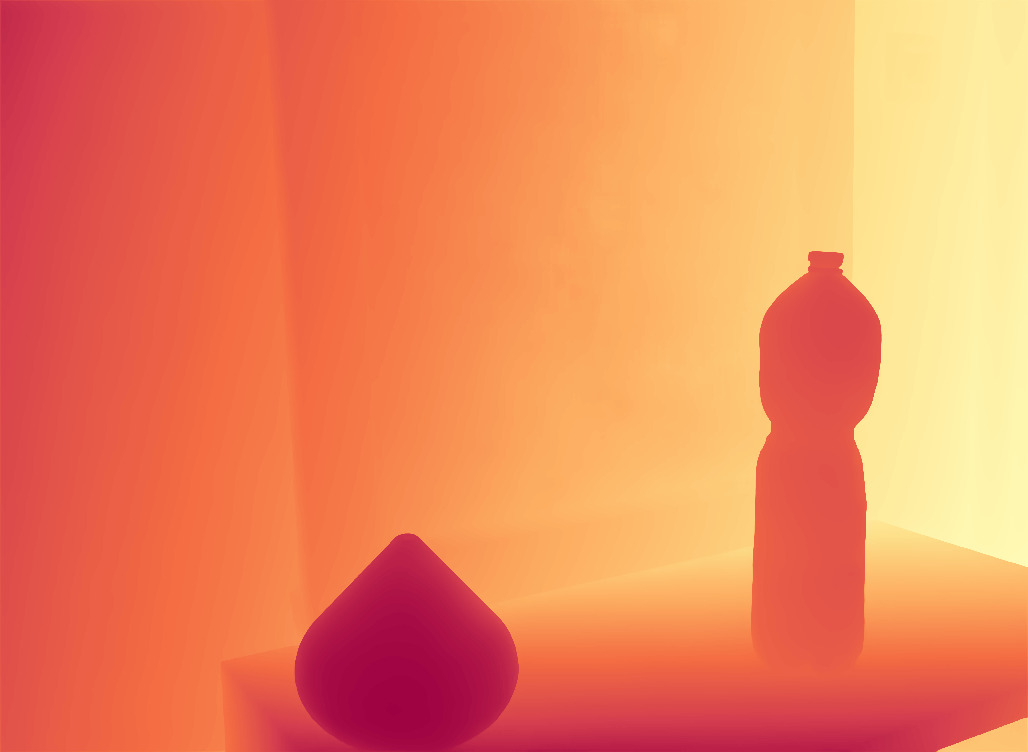
\includegraphics[width=0.3\linewidth]{imgs/mirror_with_truncation.jpg} \\

    \end{tabular}\vspace{-0.3cm}
    \caption{\textbf{Qualitative Results -- Volume Truncation.} Predictions by \method{}.}
    \label{fig:truncation}\vspace{-0.3cm}
\end{figure*}


\subsection{Runtime \& Memory Consumption Analysis}
\label{subsec:runtime}
Table \ref{tab:runtime} reports the processing time (in seconds) and memory consumption (in GB) required by \method during inference, comparing it with the baseline stereo backbone, RAFT-Stereo.
We measure the runtime on a single A100 GPU, repeating the experiment with three different input resolutions, specifically $256\times256$, $512\times512$, and $1024\times1024$, as well as by deploying the different VFMs studied before to fuel \method{} -- specifically, for each variant we report standalone runtime and memory usage by the VFM and the stereo backbone separately, as well as their sum. 

Concerning runtime, Depth Anything v2 is the fastest among the VFMs, taking about 30ms to process a single image at any resolution, with Moge requiring more than $10\times$ the time for a single inference when processing 1Mpx images. 
The stereo backbone requires about 50\% additional time compared to the baseline, RAFT-Stereo \cite{lipson2021raft}, because of the additional branch deployed to process the depth maps by the VFM.


For what concerns memory consumption, once again Depth Anything v2 is the most efficient among the VFMs, requiring as few as 2GB, with Moge sharing similar requirements. Our stereo backbone introduces additional memory consumption because of the second branch processing monocular cues: this overhead is negligible with $256\time256$ images, raising to about $2\times$ the memory required by RAFT-Stereo alone when dealing with 1Mpx images.

\begin{table}[ht]
\centering
\renewcommand{\tabcolsep}{6pt}
\scalebox{0.9}{
\begin{tabular}{|lll|rrr|rrr|}
\hline
  Image Size & Stereo Model Name & VFM Name & \multicolumn{3}{c|}{Processing Time (s)} & \multicolumn{3}{c|}{Memory Consumption (GB)} \\
  $(H \times W)$ &  &  & VFM & Stereo & Total & VFM & Stereo & Total \\
\hline\hline
\multirow{4}{*}{$256 \times 256$} & \multirow{4}{*}{\textbf{\method (ours)}} & DAv2 \cite{depth_anything_v2} & 0.03 & 0.15 & 0.18 & 0.57 & 0.18 & 0.76 \\
 & & DepthPro \cite{depthpro} & 0.21 & 0.15 & 0.36 & 1.92 & 0.18 & 2.09 \\
 & & MoGe \cite{wang2024moge} & 0.38 & 0.15 & 0.52 & 0.38 & 0.19 & 0.57 \\
 & & Lotus \cite{he2024lotus} & 0.13 & 0.15 & 0.29 & 0.22 & 0.18 & 0.41 \\
 \hline
 $256\times256$ & RAFT-Stereo \cite{lipson2021raft} & - & - & 0.10 & 0.10  & - & 0.17 & 0.17 \\
\hline\hline
 \multirow{4}{*}{$512\times512$} & \multirow{4}{*}{\textbf{\method (ours)}} & DAv2 \cite{depth_anything_v2} & 0.03 & 0.21 & 0.24 & 0.57 & 0.77 & 1.34 \\
 &  & DepthPro \cite{depthpro} & 0.20 & 0.21 & 0.41 & 1.84 & 0.77 & 2.60 \\
 &  & MoGe \cite{wang2024moge} & 0.38 & 0.21 & 0.59 & 0.38 & 0.78 & 1.17 \\
 &  & Lotus \cite{he2024lotus} & 0.16 & 0.22 & 0.38 & 0.85 & 0.77 & 1.62 \\
 \hline
 $512\times512$ & RAFT-Stereo \cite{lipson2021raft} & - & - & 0.14 & 0.14 & - & 0.66 & 0.66 \\
\hline\hline
 \multirow{4}{*}{$1024\times1024$} & \multirow{4}{*}{\textbf{\method (ours)}} & DAv2 \cite{depth_anything_v2} & 0.03 & 0.61 & 0.63 & 0.58 & 5.73 & 6.31 \\
 &  & DepthPro \cite{depthpro} & 0.21 & 0.61 & 0.82 & 1.85 & 5.73 & 7.59 \\
 &  & MoGe \cite{wang2024moge} & 0.38 & 0.60 & 0.98 & 0.42 & 5.77 & 6.19 \\
 &  & Lotus \cite{he2024lotus} & 0.49 & 0.61 & 1.10 & 3.40 & 5.73 & 9.13 \\
 \hline
 $1024\times1024$ & RAFT-Stereo \cite{lipson2021raft} & - & - & 0.36 & 0.36 & - & 2.63 & 2.63 \\
\hline
\end{tabular}}\vspace{-0.2cm}
\caption{\textbf{Runtime \& Memory Consumption Analysis.} 
}\vspace{-0.3cm}
\label{tab:runtime}
\end{table}


\clearpage

\section{Qualitative Results}
\label{subsec:qual}

We conclude with additional qualitative results by \method on the different datasets involved in our experiments.

Figure \ref{fig:qual_kitti12_1} shows two examples from the KITTI 2012 dataset (respectively, stereo pairs \textit{000040} and \textit{000068}). We can notice how any existing stereo model is unable to properly perceive the presence of transparent surfaces, as in correspondence of the windows on buildings and cars. On the contrary \method{}, driven by the priors injected through the VFM, properly predicts the disparity corresponding to the transparent surfaces.   

\begin{figure*}[h]
    \centering 
    \renewcommand{\tabcolsep}{1pt}
    \begin{tabular}{cc}

        \small RGB &
        \small RAFT-Stereo \cite{lipson2021raft} \\
        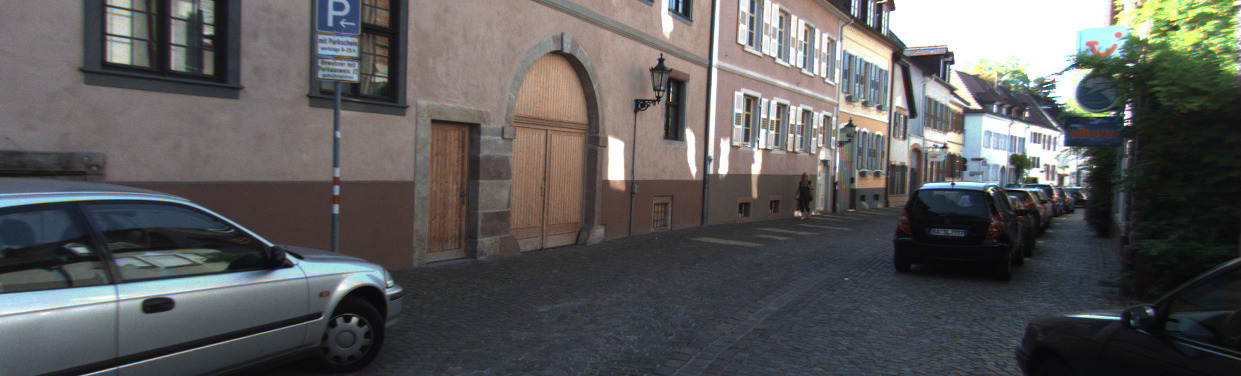
\includegraphics[width=0.48\textwidth]{imgs/KITTI12/rgb/40.jpg} & 
        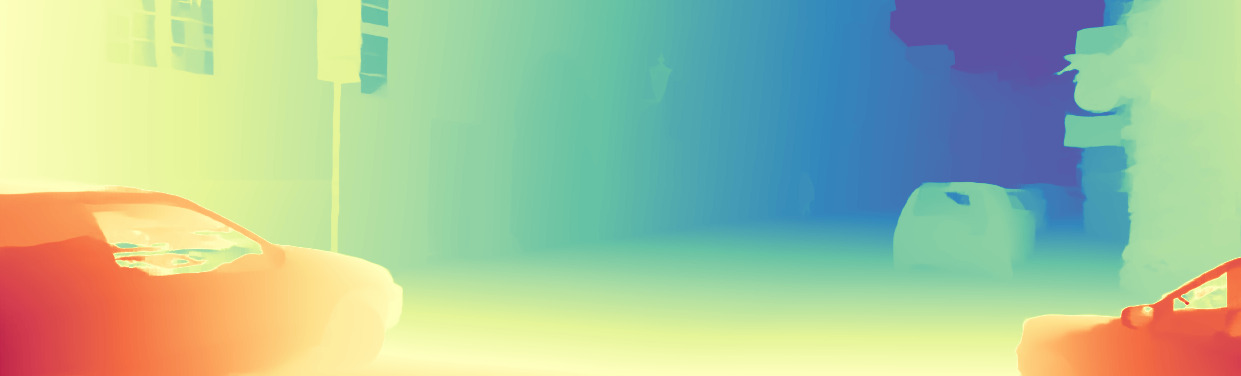
\includegraphics[width=0.48\textwidth]{imgs/KITTI12/stereo/RAFT-Stereo/40.jpg} \\
        \small DLNR \cite{zhao2023high} &
        \small NMRF \cite{guan2024neural} \\
        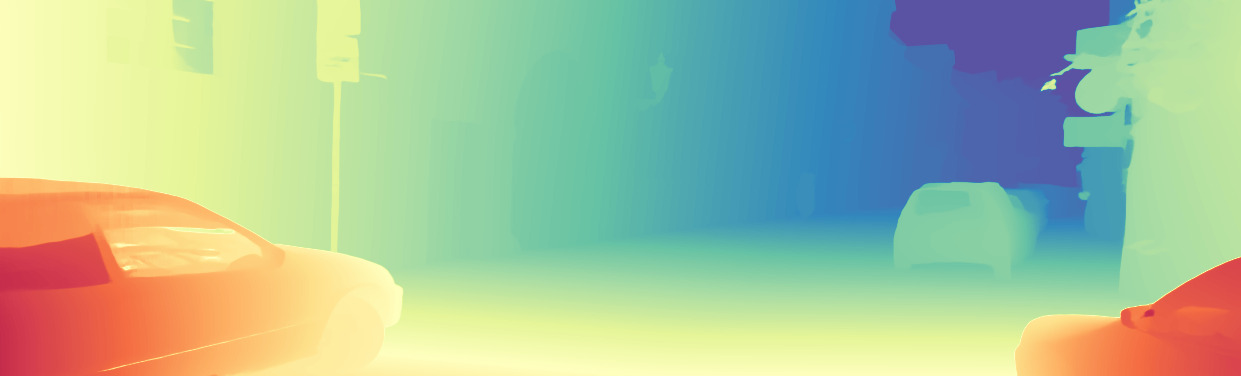
\includegraphics[width=0.48\textwidth]{imgs/KITTI12/stereo/DLNR/40.jpg} &
        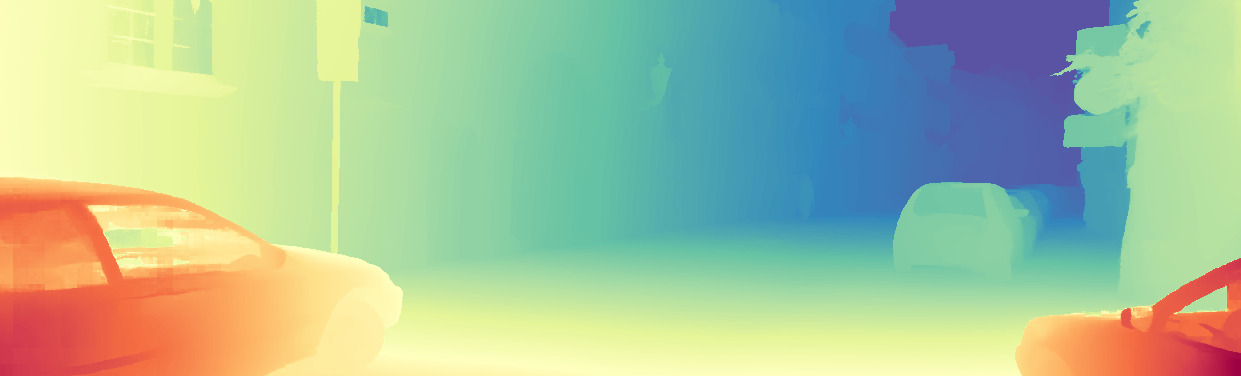
\includegraphics[width=0.48\textwidth]{imgs/KITTI12/stereo/NMRF/40.jpg} \\ 
        \small Selective-IGEV \cite{wang2024selective} &
        \textbf{\method (ours)} \\
        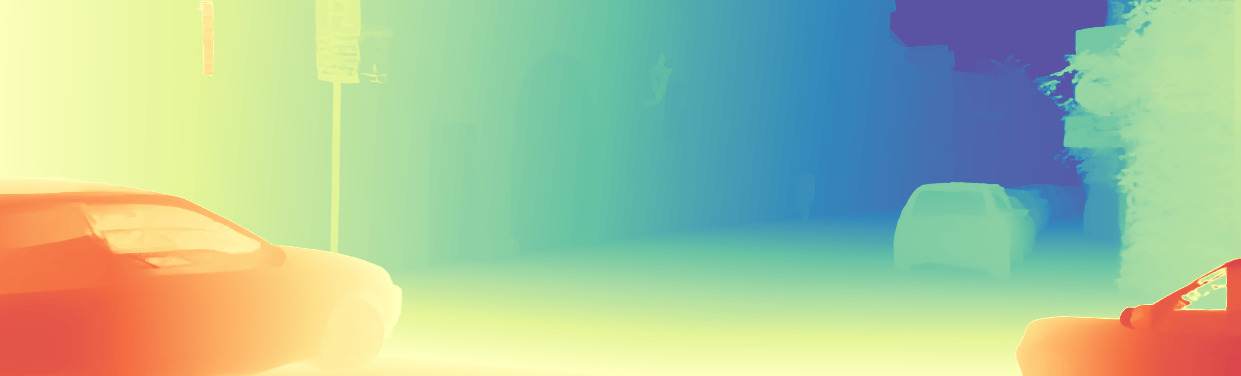
\includegraphics[width=0.48\textwidth]{imgs/KITTI12/stereo/Selective/40.jpg} &
        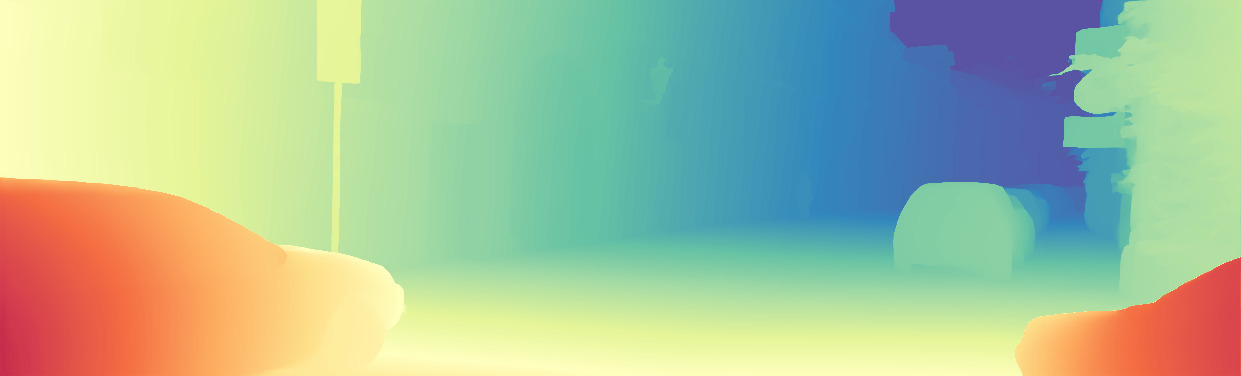
\includegraphics[width=0.48\textwidth]{imgs/KITTI12/stereo/Ours/40.jpg} \\ \\

        \small RGB &
        \small RAFT-Stereo \cite{lipson2021raft} \\
        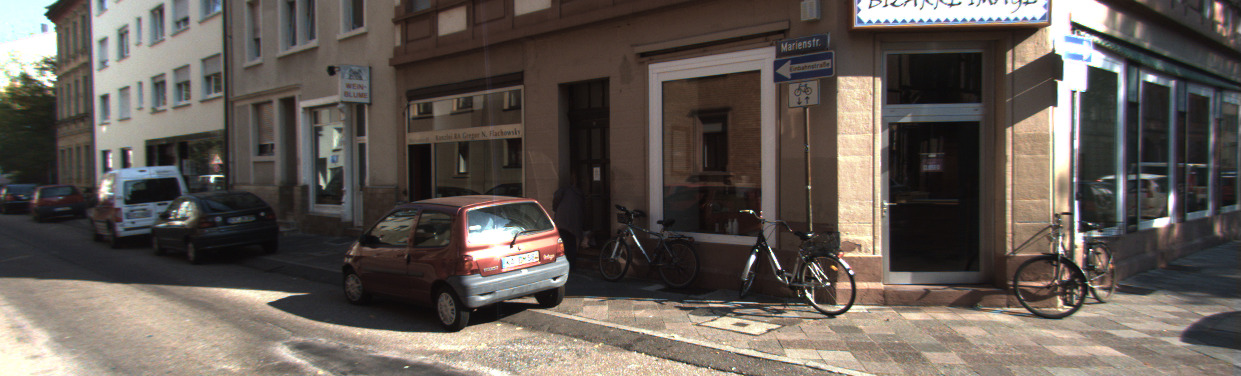
\includegraphics[width=0.48\textwidth]{imgs/KITTI12/rgb/68.jpg} & 
        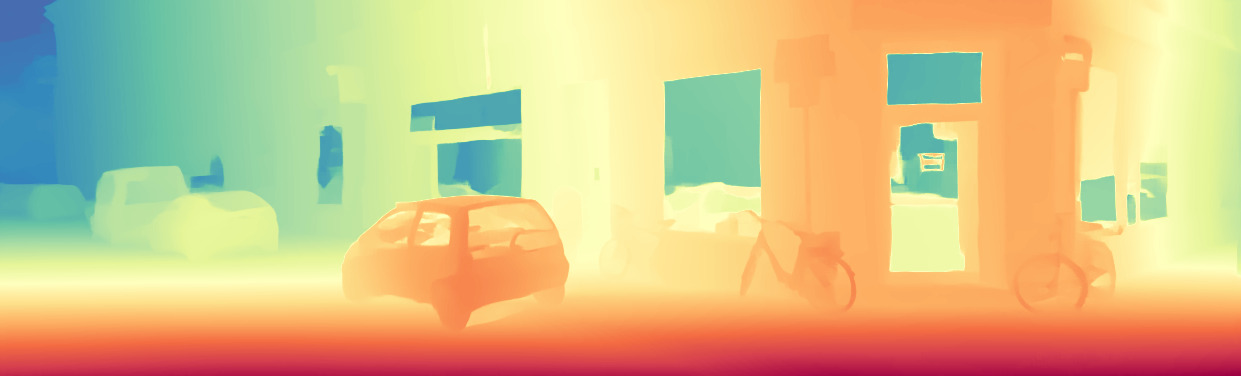
\includegraphics[width=0.48\textwidth]{imgs/KITTI12/stereo/RAFT-Stereo/68.jpg} \\
        \small DLNR \cite{zhao2023high} &
        \small NMRF \cite{guan2024neural} \\
        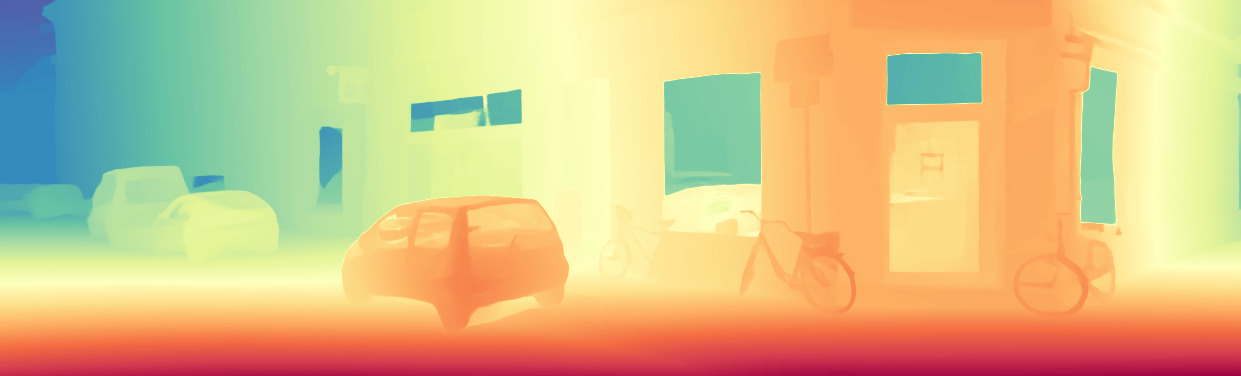
\includegraphics[width=0.48\textwidth]{imgs/KITTI12/stereo/DLNR/68.jpg} &
        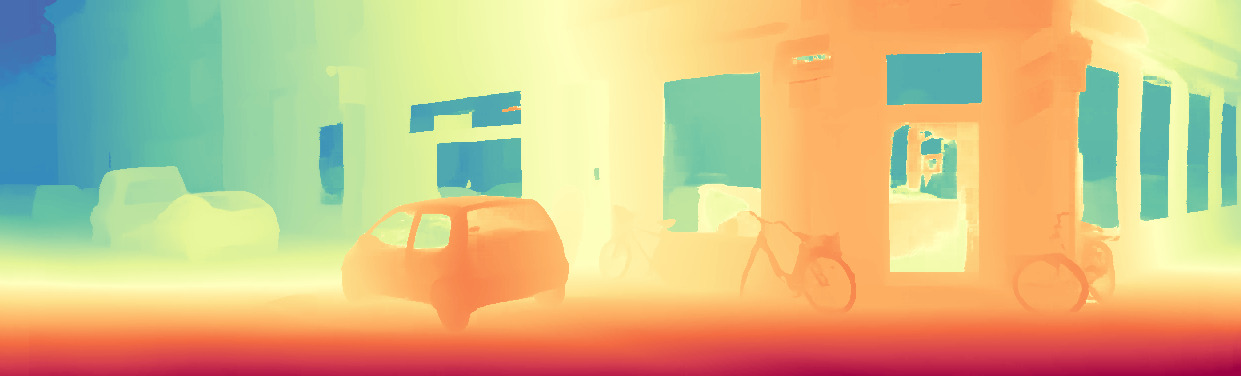
\includegraphics[width=0.48\textwidth]{imgs/KITTI12/stereo/NMRF/68.jpg} \\ 
        \small Selective-IGEV \cite{wang2024selective} &
        \textbf{\method (ours)} \\
        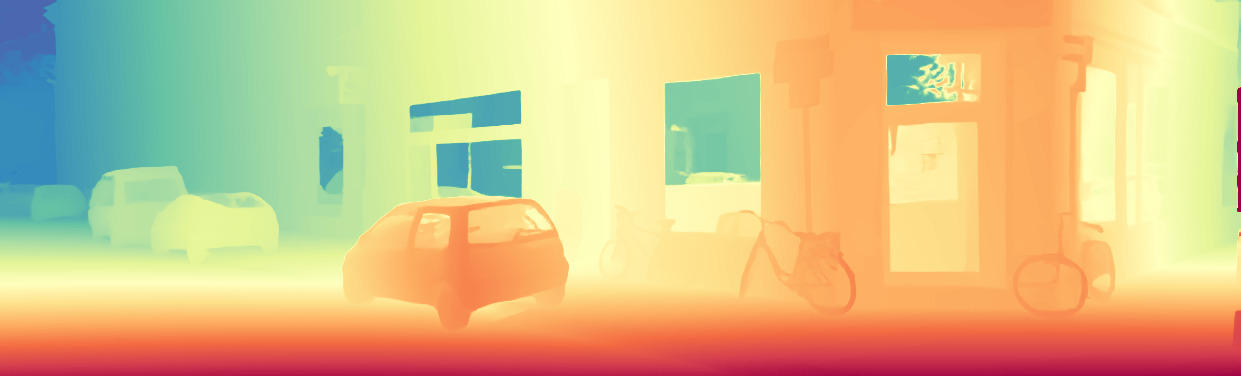
\includegraphics[width=0.48\textwidth]{imgs/KITTI12/stereo/Selective/68.jpg} &
        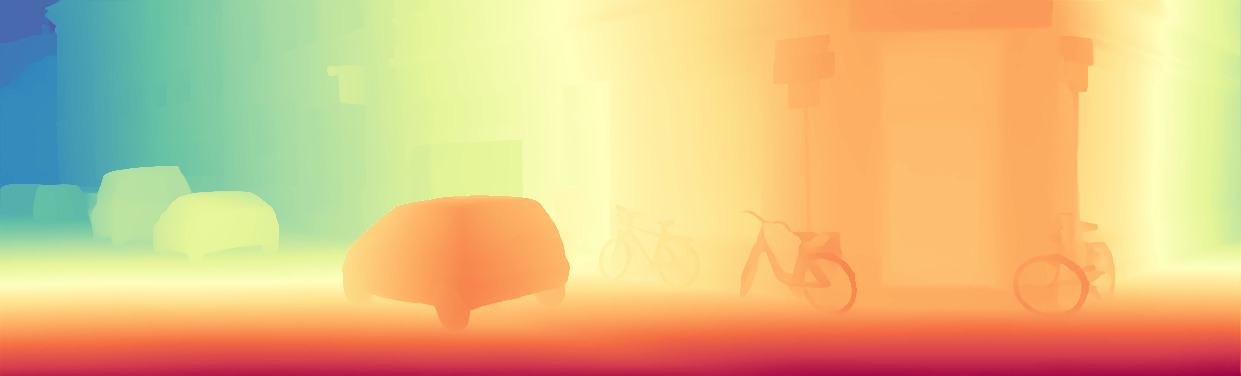
\includegraphics[width=0.48\textwidth]{imgs/KITTI12/stereo/Ours/68.jpg} \\ 
    \end{tabular}\vspace{-0.3cm}
    \caption{\textbf{Qualitative Results -- KITTI 2012 (part 1).} Predictions by state-of-the-art models and \method.}
    \label{fig:qual_kitti12_1}\vspace{-0.3cm}
\end{figure*}

\clearpage

Figure \ref{fig:qual_kitti12_2} shows two further examples from KITTI 2012 (respectively, stereo pairs \textit{000073} and \textit{000127}). In this case, we can appreciate the much higher level of detail in the disparity maps predicted by \method, with extremely thin structures in fences and gates being preserved.

\begin{figure*}[h]
    \centering 
    \renewcommand{\tabcolsep}{1pt}
    \begin{tabular}{cc}
        \small RGB &
        \small RAFT-Stereo \cite{lipson2021raft} \\
        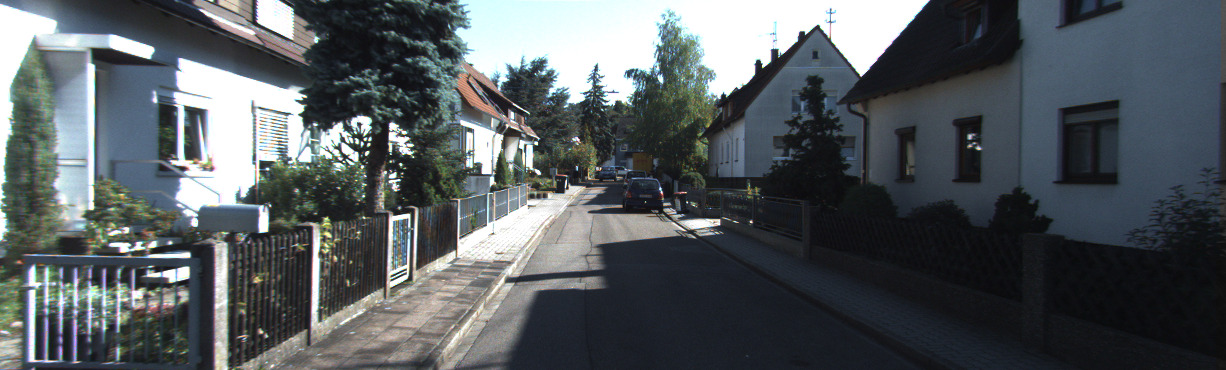
\includegraphics[width=0.48\textwidth]{imgs/KITTI12/rgb/73.jpg} & 
        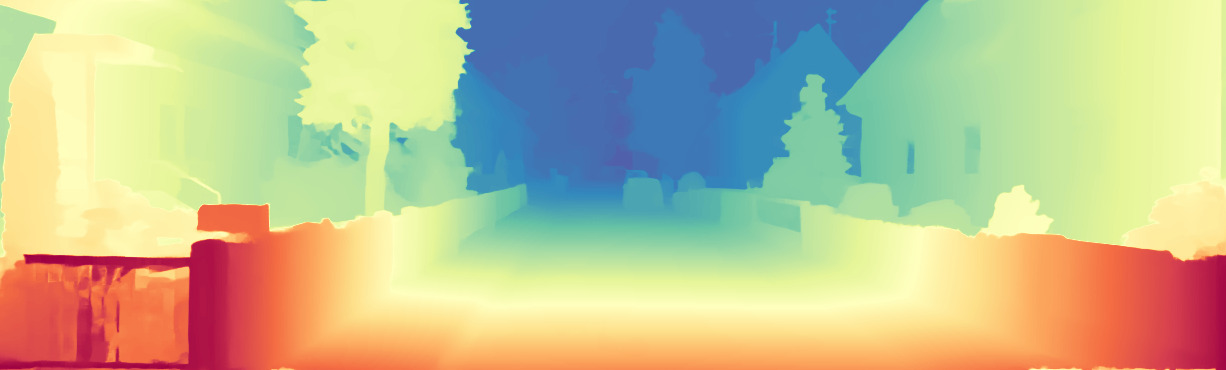
\includegraphics[width=0.48\textwidth]{imgs/KITTI12/stereo/RAFT-Stereo/73.jpg} \\
        \small DLNR \cite{zhao2023high} &
        \small NMRF \cite{guan2024neural} \\
        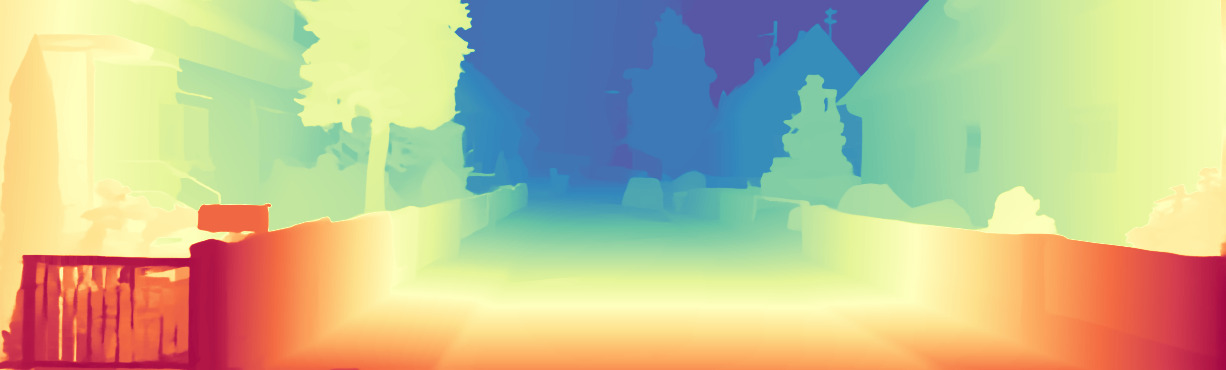
\includegraphics[width=0.48\textwidth]{imgs/KITTI12/stereo/DLNR/73.jpg} &
        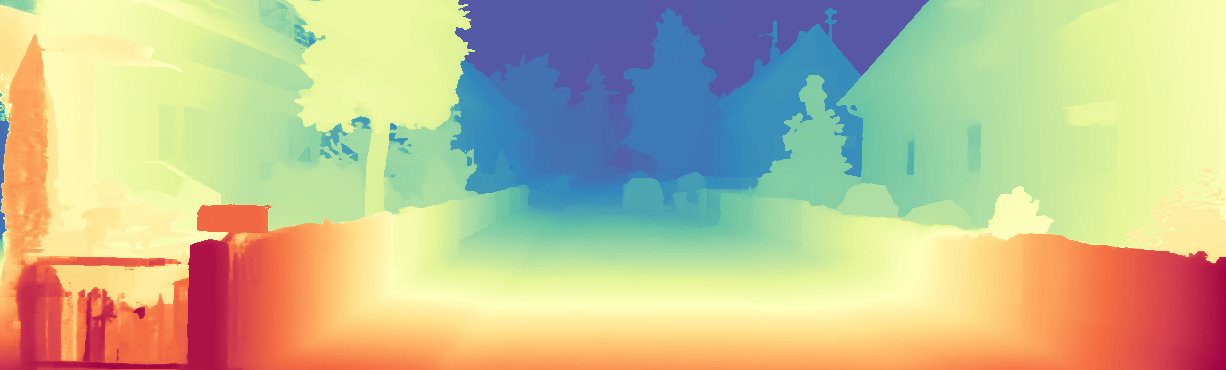
\includegraphics[width=0.48\textwidth]{imgs/KITTI12/stereo/NMRF/73.jpg} \\ 
        \small Selective-IGEV \cite{wang2024selective} &
        \textbf{\method (ours)} \\
        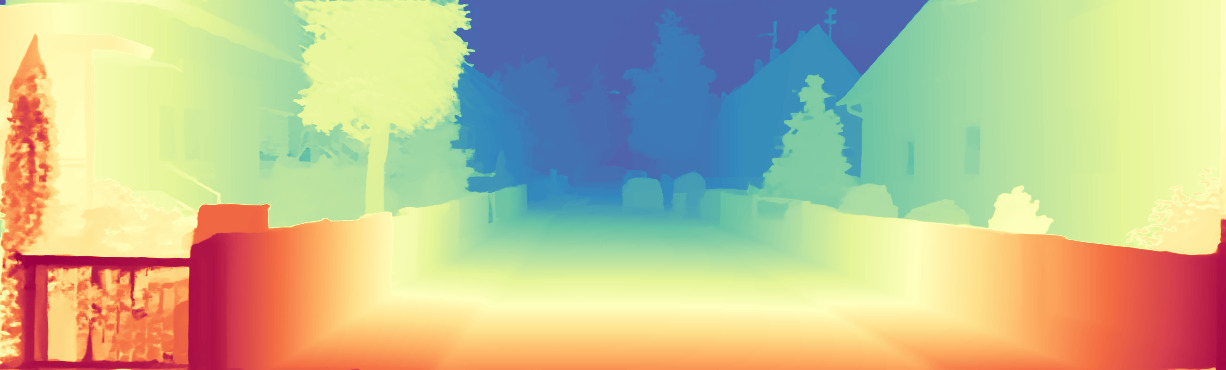
\includegraphics[width=0.48\textwidth]{imgs/KITTI12/stereo/Selective/73.jpg} &
        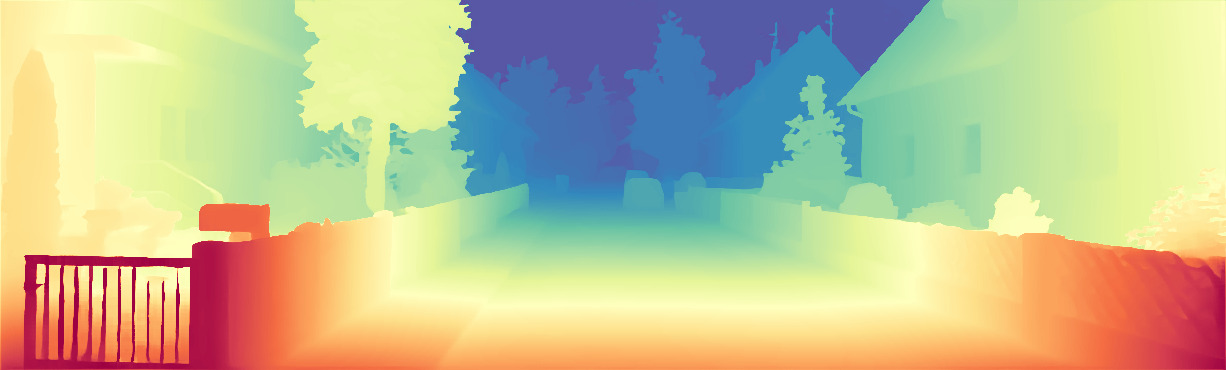
\includegraphics[width=0.48\textwidth]{imgs/KITTI12/stereo/Ours/73.jpg} \\ \\

        \small RGB &
        \small RAFT-Stereo \cite{lipson2021raft} \\
        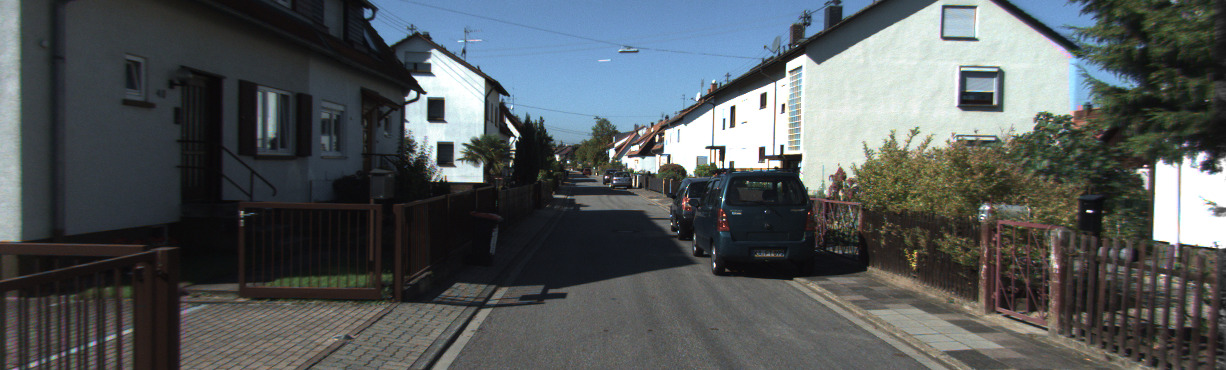
\includegraphics[width=0.48\textwidth]{imgs/KITTI12/rgb/127.jpg} & 
        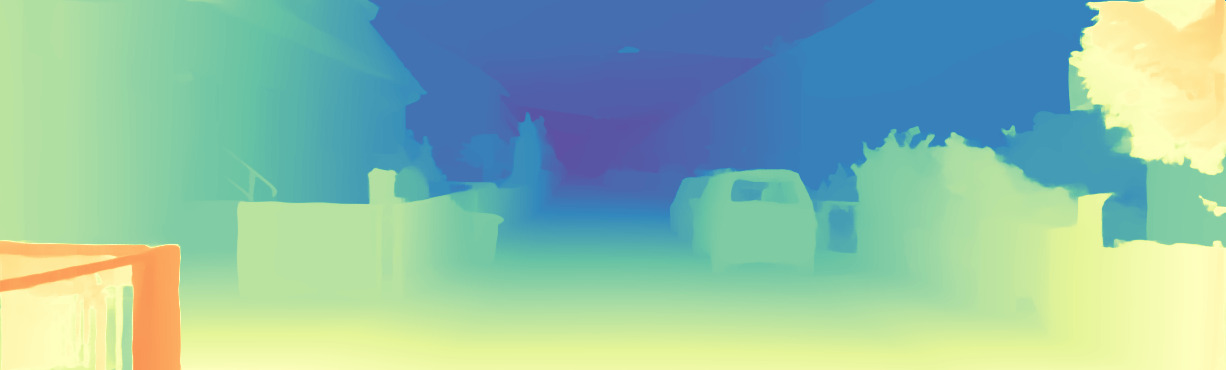
\includegraphics[width=0.48\textwidth]{imgs/KITTI12/stereo/RAFT-Stereo/127.jpg} \\
        \small DLNR \cite{zhao2023high} &
        \small NMRF \cite{guan2024neural} \\
        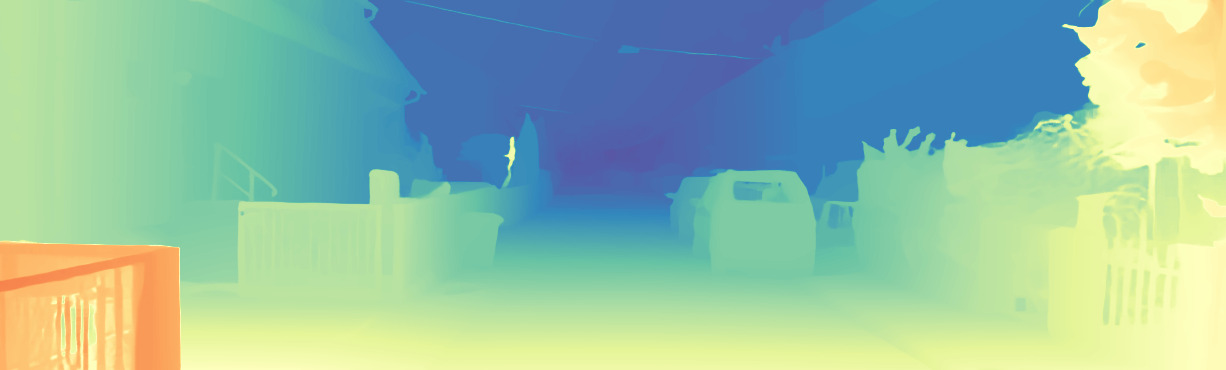
\includegraphics[width=0.48\textwidth]{imgs/KITTI12/stereo/DLNR/127.jpg} &
        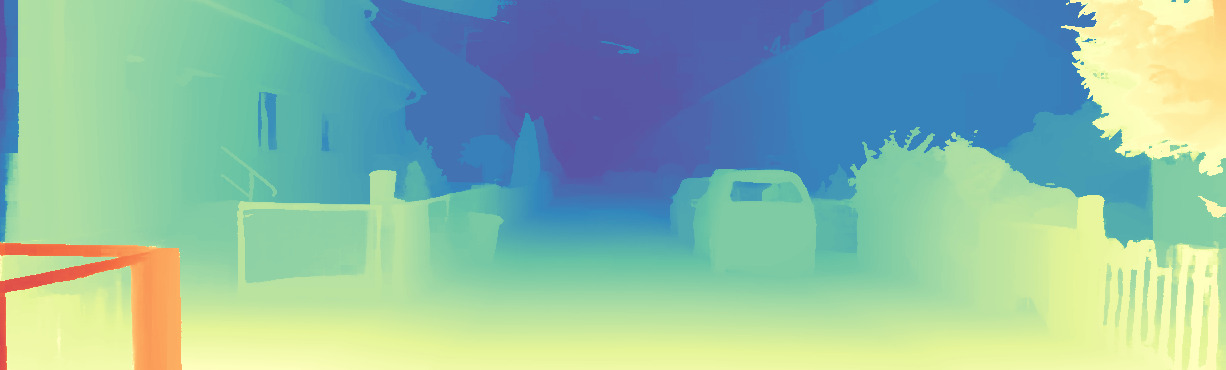
\includegraphics[width=0.48\textwidth]{imgs/KITTI12/stereo/NMRF/127.jpg} \\ 
        \small Selective-IGEV \cite{wang2024selective} &
        \textbf{\method (ours)} \\
        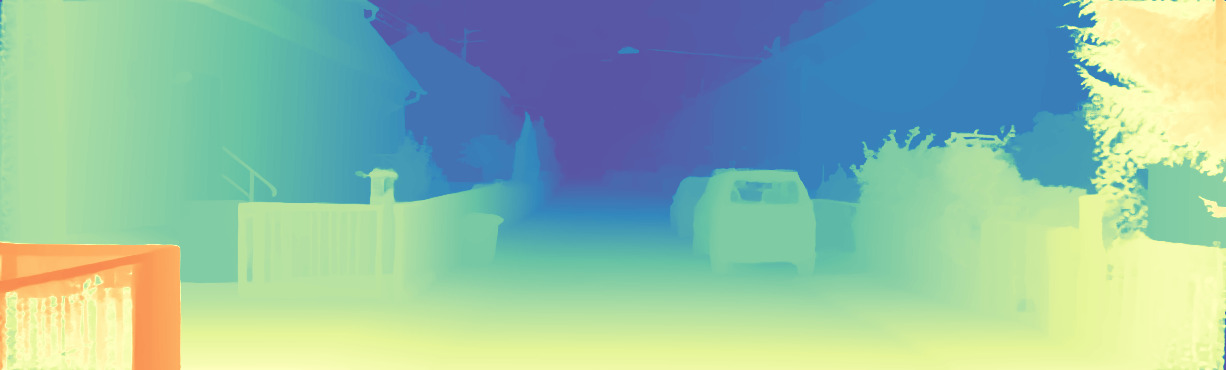
\includegraphics[width=0.48\textwidth]{imgs/KITTI12/stereo/Selective/127.jpg} &
        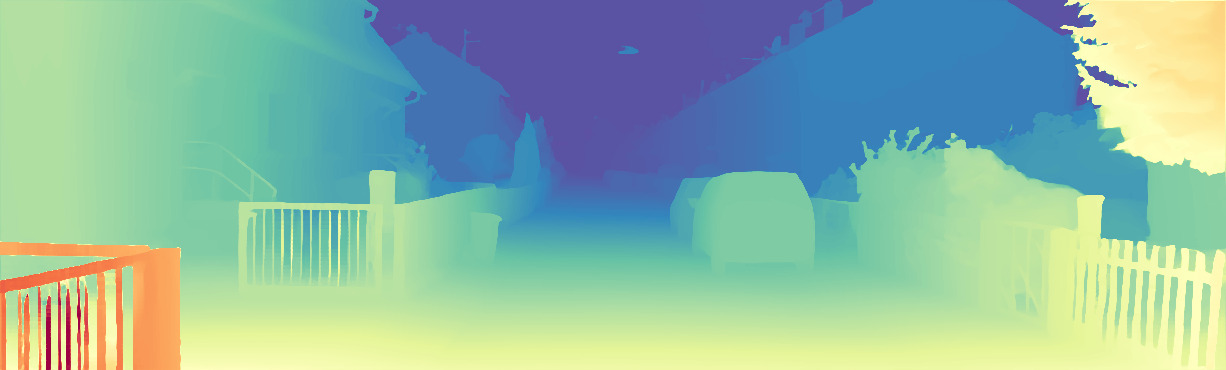
\includegraphics[width=0.48\textwidth]{imgs/KITTI12/stereo/Ours/127.jpg} \\ 
    \end{tabular}\vspace{-0.3cm}
    \caption{\textbf{Qualitative Results -- KITTI 2012 (part 2).} Predictions by state-of-the-art models and \method.}
    \label{fig:qual_kitti12_2}\vspace{-0.3cm}
\end{figure*}

\clearpage

Figure \ref{fig:qual_kitti15_1} reports two stereo pairs from KITTI 2015 (respectively, \textit{000024} and \textit{000049}). These examples confirm the ability to recover both thin structures and transparent surfaces already appreciated in KITTI 2012.

\begin{figure*}[h]
    \centering 
    \renewcommand{\tabcolsep}{1pt}
    \begin{tabular}{cc}

        \small RGB &
        \small RAFT-Stereo \cite{lipson2021raft} \\
        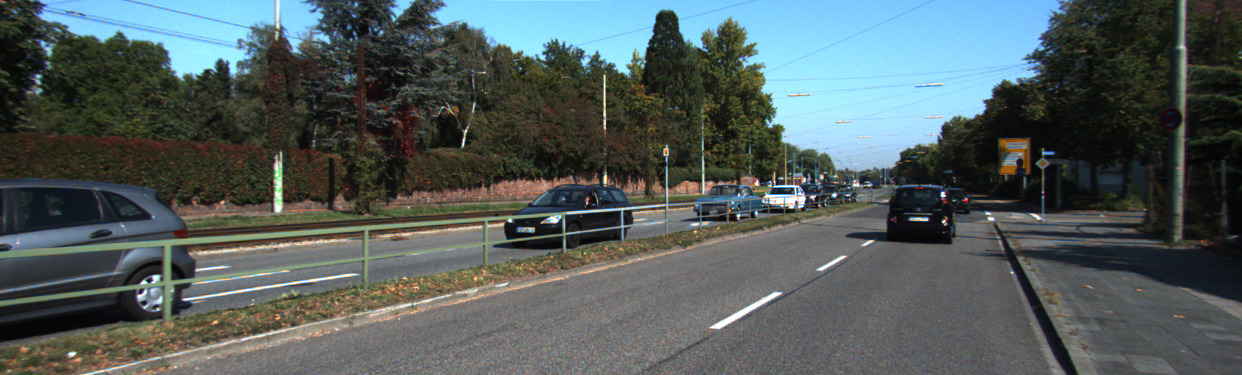
\includegraphics[width=0.48\textwidth]{imgs/KITTI/rgb/24.jpg} & 
        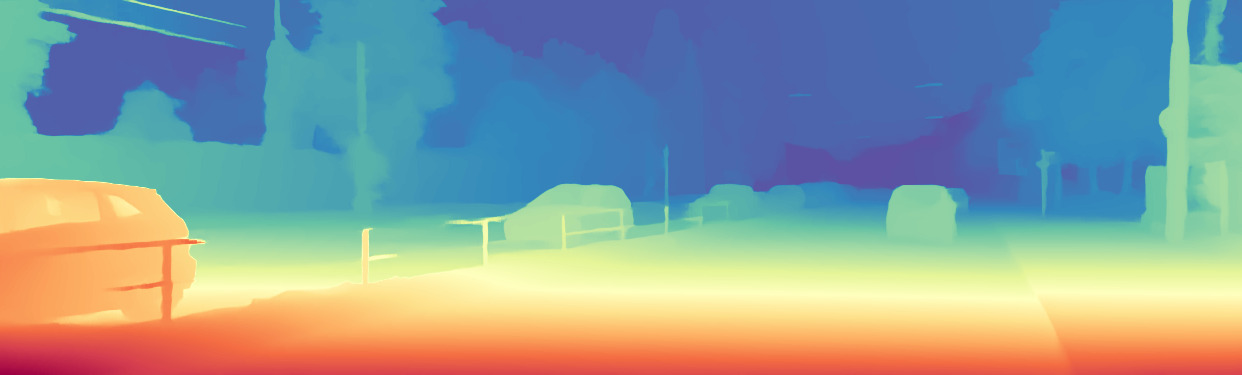
\includegraphics[width=0.48\textwidth]{imgs/KITTI/stereo/RAFT-Stereo/24.jpg} \\
        \small DLNR \cite{zhao2023high} &
        \small NMRF \cite{guan2024neural} \\
        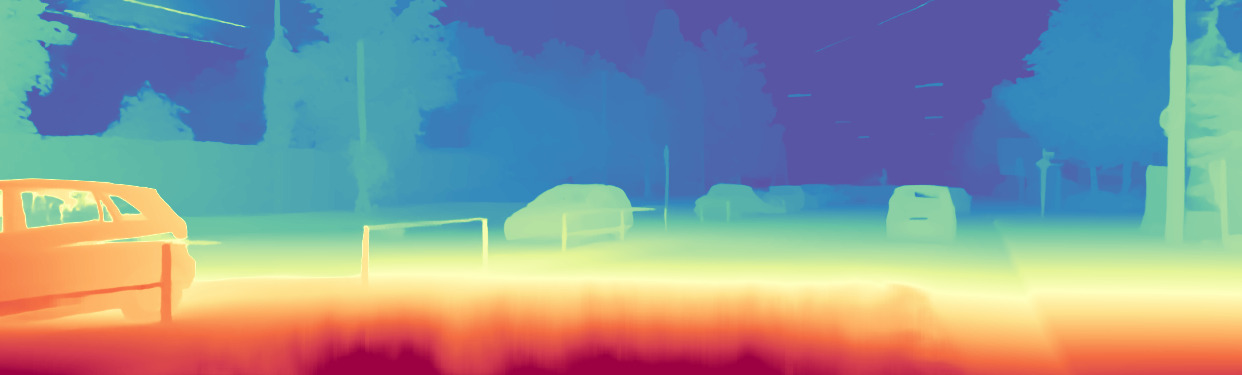
\includegraphics[width=0.48\textwidth]{imgs/KITTI/stereo/DLNR/24.jpg} &
        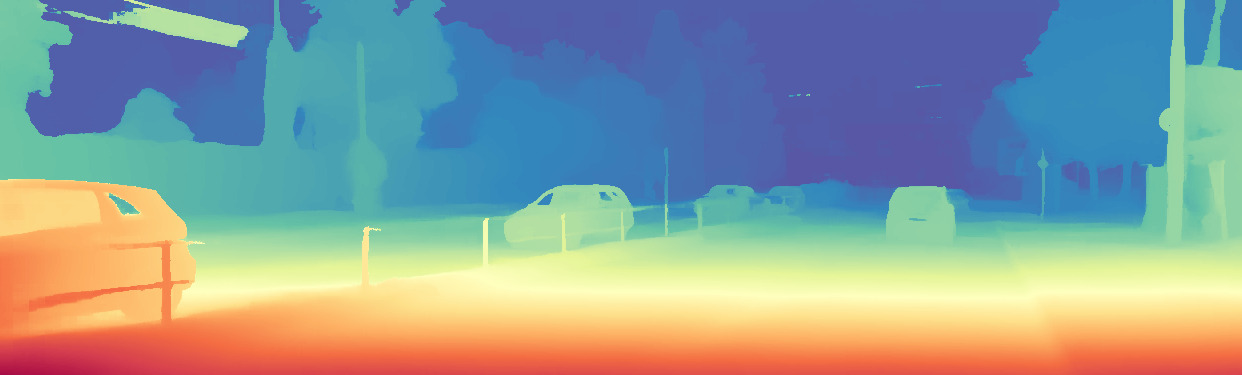
\includegraphics[width=0.48\textwidth]{imgs/KITTI/stereo/NMRF/24.jpg} \\ 
        \small Selective-IGEV \cite{wang2024selective} &
        \textbf{\method (ours)} \\
        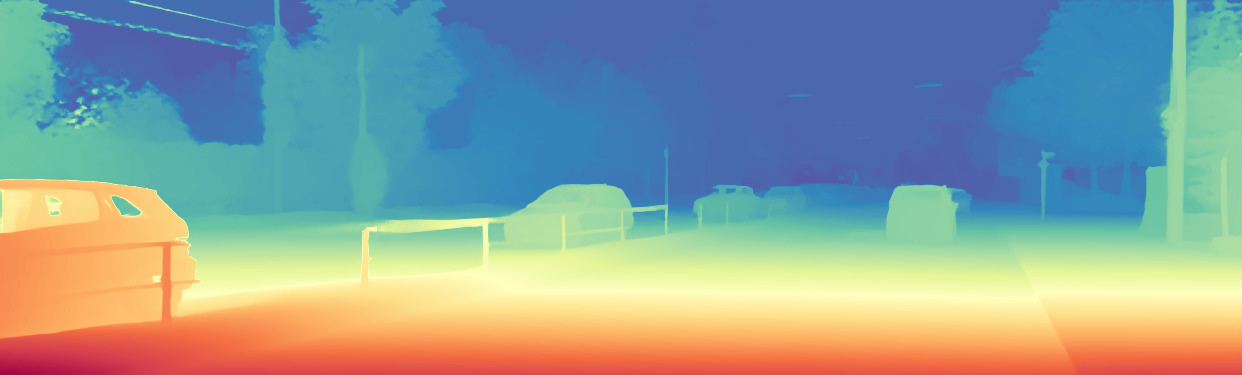
\includegraphics[width=0.48\textwidth]{imgs/KITTI/stereo/Selective/24.jpg} &
        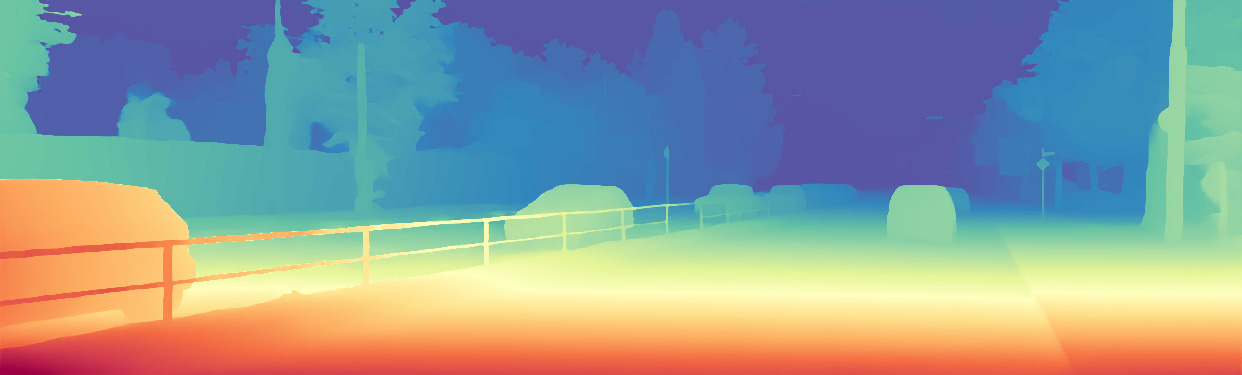
\includegraphics[width=0.48\textwidth]{imgs/KITTI/stereo/Ours/24.jpg} \\ \\

        \small RGB &
        \small RAFT-Stereo \cite{lipson2021raft} \\
        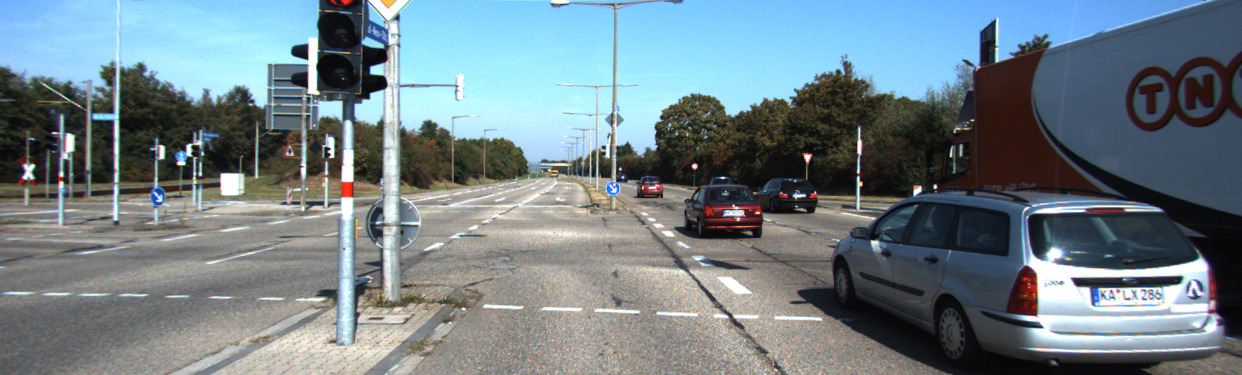
\includegraphics[width=0.48\textwidth]{imgs/KITTI/rgb/49.jpg} & 
        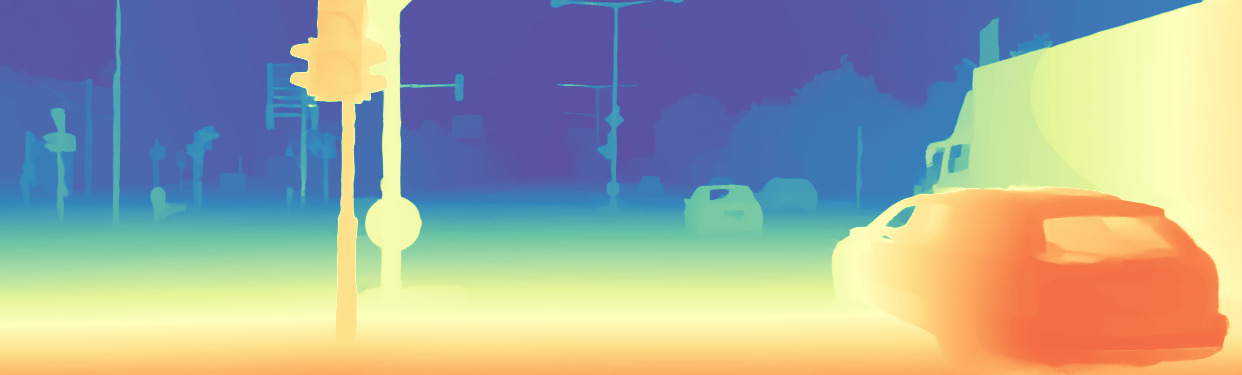
\includegraphics[width=0.48\textwidth]{imgs/KITTI/stereo/RAFT-Stereo/49.jpg} \\
        \small DLNR \cite{zhao2023high} &
        \small NMRF \cite{guan2024neural} \\
        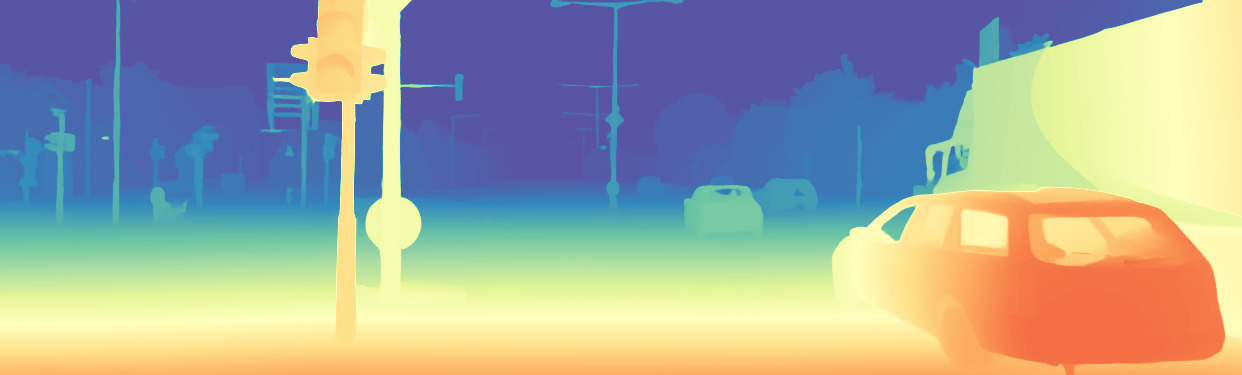
\includegraphics[width=0.48\textwidth]{imgs/KITTI/stereo/DLNR/49.jpg} &
        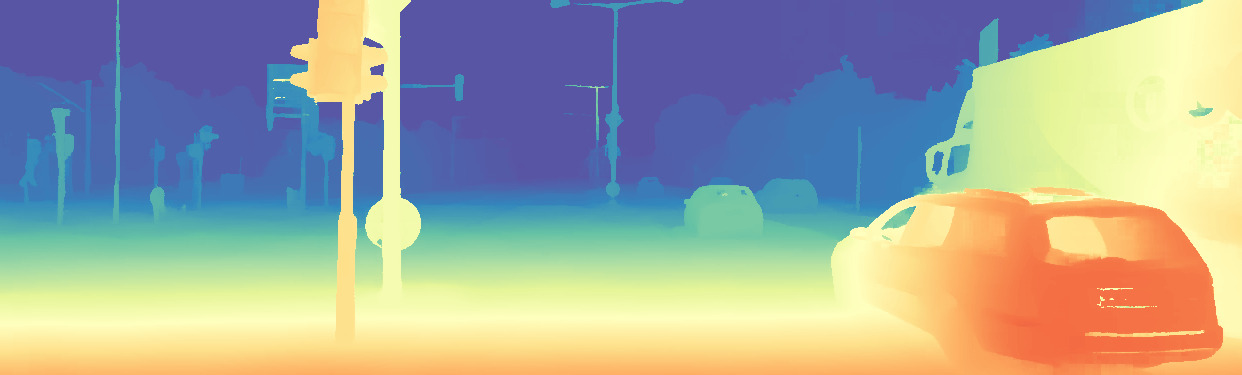
\includegraphics[width=0.48\textwidth]{imgs/KITTI/stereo/NMRF/49.jpg} \\ 
        \small Selective-IGEV \cite{wang2024selective} &
        \textbf{\method (ours)} \\
        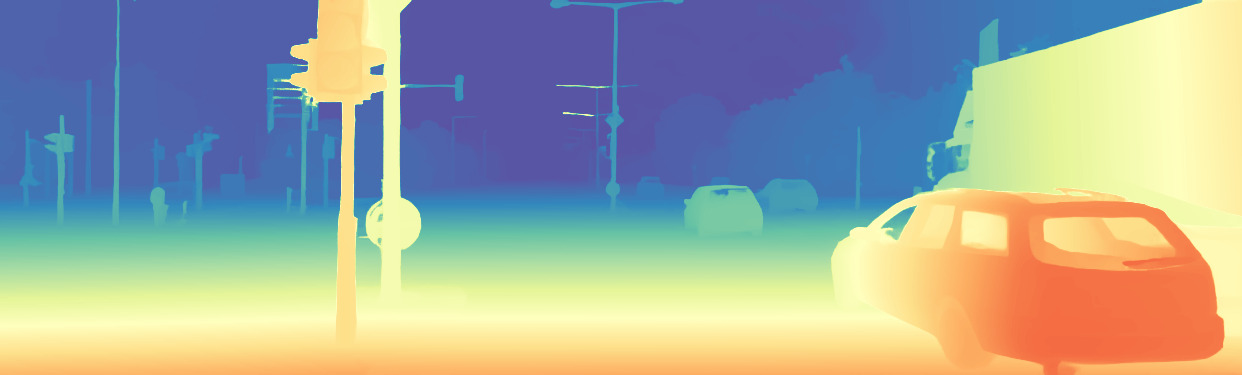
\includegraphics[width=0.48\textwidth]{imgs/KITTI/stereo/Selective/49.jpg} &
        \includegraphics[width=0.48\textwidth]{imgs/KITTI/stereo/Ours/49.jpg} \\ 
    \end{tabular}\vspace{-0.3cm}
    \caption{\textbf{Qualitative Results -- KITTI 2015 (part 1).} Predictions by state-of-the-art models and \method.}
    \label{fig:qual_kitti15_1}\vspace{-0.3cm}
\end{figure*}

\clearpage

Figure \ref{fig:qual_kitti15_2} reports two additional samples from KITTI 2015 (respectively, \textit{000093} and \textit{000144}). These latter present both underexposed and transparent regions, respectively on the billboard and the tram in the two images. While existing stereo networks struggle at dealing with both, \method exposes unprecedented robustness. 

\begin{figure*}[h]
    \centering 
    \renewcommand{\tabcolsep}{1pt}
    \begin{tabular}{cc}
        \small RGB &
        \small RAFT-Stereo \cite{lipson2021raft} \\
        \includegraphics[width=0.48\textwidth]{imgs/KITTI/rgb/93.jpg} & 
        \includegraphics[width=0.48\textwidth]{imgs/KITTI/stereo/RAFT-Stereo/93.jpg} \\
        \small DLNR \cite{zhao2023high} &
        \small NMRF \cite{guan2024neural} \\
        \includegraphics[width=0.48\textwidth]{imgs/KITTI/stereo/DLNR/93.jpg} &
        \includegraphics[width=0.48\textwidth]{imgs/KITTI/stereo/NMRF/93.jpg} \\ 
        \small Selective-IGEV \cite{wang2024selective} &
        \textbf{\method (ours)} \\
        \includegraphics[width=0.48\textwidth]{imgs/KITTI/stereo/Selective/93.jpg} &
        \includegraphics[width=0.48\textwidth]{imgs/KITTI/stereo/Ours/93.jpg} \\ \\

        \small RGB &
        \small RAFT-Stereo \cite{lipson2021raft} \\
        \includegraphics[width=0.48\textwidth]{imgs/KITTI/rgb/144.jpg} & 
        \includegraphics[width=0.48\textwidth]{imgs/KITTI/stereo/RAFT-Stereo/144.jpg} \\
        \small DLNR \cite{zhao2023high} &
        \small NMRF \cite{guan2024neural} \\
        \includegraphics[width=0.48\textwidth]{imgs/KITTI/stereo/DLNR/144.jpg} &
        \includegraphics[width=0.48\textwidth]{imgs/KITTI/stereo/NMRF/144.jpg} \\ 
        \small Selective-IGEV \cite{wang2024selective} &
        \textbf{\method (ours)} \\
        \includegraphics[width=0.48\textwidth]{imgs/KITTI/stereo/Selective/144.jpg} &
        \includegraphics[width=0.48\textwidth]{imgs/KITTI/stereo/Ours/144.jpg} \\ 
    \end{tabular}\vspace{-0.3cm}
    \caption{\textbf{Qualitative Results -- KITTI 2015 (part 2).} Predictions by state-of-the-art models and \method.}
    \label{fig:qual_kitti15_2}\vspace{-0.3cm}
\end{figure*}

\clearpage

Figure \ref{fig:qual_midd14} reports two image pairs from Middlebury 2014 (respectively, \textit{Adirondack} and \textit{Vintage}). On the former, \method preserves the very thin holes on the back of the chair, while on the latter it can properly estimate the disparity for the displays, where existing methods are fooled and predict holes.

\begin{figure*}[h]
    \centering
    \renewcommand{\tabcolsep}{1pt}
    \begin{tabular}{ccc}
        \small RGB &
        \small RAFT-Stereo \cite{lipson2021raft} &
        \small DLNR \cite{zhao2023high} \\
        \includegraphics[width=0.32\textwidth]{imgs/middlebury/rgb/0.jpg} & 
        \includegraphics[width=0.32\textwidth]{imgs/middlebury/stereo/RAFT-Stereo/0.jpg} &
        \includegraphics[width=0.32\textwidth]{imgs/middlebury/stereo/DLNR/0.jpg} \\
        \small NMRF \cite{guan2024neural} &
        \small Selective-IGEV \cite{wang2024selective} &
        \textbf{\method (ours)} \\
        \includegraphics[width=0.32\textwidth]{imgs/middlebury/stereo/NMRF/0.jpg} &
        \includegraphics[width=0.32\textwidth]{imgs/middlebury/stereo/Selective/0.jpg} &
        \includegraphics[width=0.32\textwidth]{imgs/middlebury/stereo/Ours/0.jpg} \\ \\
        
        \small RGB &
        \small RAFT-Stereo \cite{lipson2021raft} &
        \small DLNR \cite{zhao2023high} \\
        \includegraphics[width=0.32\textwidth]{imgs/middlebury/rgb/14.jpg} & 
        \includegraphics[width=0.32\textwidth]{imgs/middlebury/stereo/RAFT-Stereo/14.jpg} &
        \includegraphics[width=0.32\textwidth]{imgs/middlebury/stereo/DLNR/14.jpg} \\
        \small NMRF \cite{guan2024neural} &
        \small Selective-IGEV \cite{wang2024selective} &
        \textbf{\method (ours)} \\
        \includegraphics[width=0.32\textwidth]{imgs/middlebury/stereo/NMRF/14.jpg} &
        \includegraphics[width=0.32\textwidth]{imgs/middlebury/stereo/Selective/14.jpg} &
        \includegraphics[width=0.32\textwidth]{imgs/middlebury/stereo/Ours/14.jpg} \\ 
    \end{tabular}\vspace{-0.3cm}
    \caption{\textbf{Qualitative Results -- Middlebury 2014.} Predictions by state-of-the-art models and \method.}
    \label{fig:qual_midd14}\vspace{-0.3cm}
\end{figure*}

\clearpage

Figure \ref{fig:qual_midd21_1} and \ref{fig:qual_midd21_2} shows the results on two samples from Middlebury 2021, peculiar for their aspect ratio (respectively, \textit{ladder1} and \textit{ladder2}). Although existing models perform quite well on both, they fail to preserve the skittles on the top of the scene, whereas \method properly predicts their structure.

\begin{figure*}[h]
    \centering
    \renewcommand{\tabcolsep}{1pt}
    \begin{tabular}{ccc}
        \small RGB &
        \small RAFT-Stereo \cite{lipson2021raft} &
        \small DLNR \cite{zhao2023high} \\
        \includegraphics[width=0.3\textwidth]{imgs/midd21/rgb/10.jpg} & 
        \includegraphics[width=0.3\textwidth]{imgs/midd21/stereo/RAFT-Stereo/10.jpg} &
        \includegraphics[width=0.3\textwidth]{imgs/midd21/stereo/DLNR/10.jpg} \\
        \small NMRF \cite{guan2024neural} &
        \small Selective-IGEV \cite{wang2024selective} &
        \textbf{\method (ours)} \\
        \includegraphics[width=0.3\textwidth]{imgs/midd21/stereo/NMRF/10.jpg} &
        \includegraphics[width=0.3\textwidth]{imgs/midd21/stereo/Selective/10.jpg} &
        \includegraphics[width=0.3\textwidth]{imgs/midd21/stereo/Ours/10.jpg} \\ 
    \end{tabular}\vspace{-0.3cm}
    \caption{\textbf{Qualitative Results -- Middlebury 2021 (part 1).} Predictions by state-of-the-art models and \method.}
    \label{fig:qual_midd21_1}\vspace{-0.3cm}
\end{figure*}

\clearpage

\begin{figure*}[h]
    \centering
    \renewcommand{\tabcolsep}{1pt}
    \begin{tabular}{ccc}
        \small RGB &
        \small RAFT-Stereo \cite{lipson2021raft} &
        \small DLNR \cite{zhao2023high} \\
        \includegraphics[width=0.3\textwidth]{imgs/midd21/rgb/11.jpg} & 
        \includegraphics[width=0.3\textwidth]{imgs/midd21/stereo/RAFT-Stereo/11.jpg} &
        \includegraphics[width=0.3\textwidth]{imgs/midd21/stereo/DLNR/11.jpg} \\
        \small NMRF \cite{guan2024neural} &
        \small Selective-IGEV \cite{wang2024selective} &
        \textbf{\method (ours)} \\
        \includegraphics[width=0.3\textwidth]{imgs/midd21/stereo/NMRF/11.jpg} &
        \includegraphics[width=0.3\textwidth]{imgs/midd21/stereo/Selective/11.jpg} &
        \includegraphics[width=0.3\textwidth]{imgs/midd21/stereo/Ours/11.jpg} \\ 
    \end{tabular}\vspace{-0.3cm}
    \caption{\textbf{Qualitative Results -- Middlebury 2021 (part 2).} Predictions by state-of-the-art models and \method.}
    \label{fig:qual_midd21_2}\vspace{-0.3cm}
\end{figure*}

\clearpage

Figure \ref{fig:qual_eth3d} collects three outdoor images from ETH3D (respectively, \textit{Playground1}, \textit{Playground2} and \textit{Playground3}). Once again, \method proves its supremacy at predicting fine details such as branches and poles, while resulting more robust to challenging illumination conditions such as the sun flare in \textit{Playground2}.

\begin{figure*}[h]
    \centering
    \renewcommand{\tabcolsep}{1pt}
    \begin{tabular}{ccc}
        \small RGB &
        \small RAFT-Stereo \cite{lipson2021raft} &
        \small DLNR \cite{zhao2023high} \\
        \includegraphics[width=0.31\textwidth]{imgs/ETH3D/rgb/15.jpg} & 
        \includegraphics[width=0.31\textwidth]{imgs/ETH3D/stereo/RAFT-Stereo/15.jpg} &
        \includegraphics[width=0.31\textwidth]{imgs/ETH3D/stereo/DLNR/15.jpg} \\
        \small NMRF \cite{guan2024neural} &
        \small Selective-IGEV \cite{wang2024selective} &
        \textbf{\method (ours)} \\
        \includegraphics[width=0.31\textwidth]{imgs/ETH3D/stereo/NMRF/15.jpg} &
        \includegraphics[width=0.31\textwidth]{imgs/ETH3D/stereo/Selective/15.jpg} &
        \includegraphics[width=0.31\textwidth]{imgs/ETH3D/stereo/Ours/15.jpg} \\ \\
        \small RGB &
        \small RAFT-Stereo \cite{lipson2021raft} &
        \small DLNR \cite{zhao2023high} \\
        \includegraphics[width=0.31\textwidth]{imgs/ETH3D/rgb/17.jpg} & 
        \includegraphics[width=0.31\textwidth]{imgs/ETH3D/stereo/RAFT-Stereo/17.jpg} &
        \includegraphics[width=0.31\textwidth]{imgs/ETH3D/stereo/DLNR/17.jpg} \\
        \small NMRF \cite{guan2024neural} &
        \small Selective-IGEV \cite{wang2024selective} &
        \textbf{\method (ours)} \\
        \includegraphics[width=0.31\textwidth]{imgs/ETH3D/stereo/NMRF/17.jpg} &
        \includegraphics[width=0.31\textwidth]{imgs/ETH3D/stereo/Selective/17.jpg} &
        \includegraphics[width=0.31\textwidth]{imgs/ETH3D/stereo/Ours/17.jpg} \\ \\

        \small RGB &
        \small RAFT-Stereo \cite{lipson2021raft} &
        \small DLNR \cite{zhao2023high} \\
        \includegraphics[width=0.31\textwidth]{imgs/ETH3D/rgb/19.jpg} & 
        \includegraphics[width=0.31\textwidth]{imgs/ETH3D/stereo/RAFT-Stereo/19.jpg} &
        \includegraphics[width=0.31\textwidth]{imgs/ETH3D/stereo/DLNR/19.jpg} \\
        \includegraphics[width=0.31\textwidth]{imgs/ETH3D/stereo/NMRF/19.jpg} &
        \includegraphics[width=0.31\textwidth]{imgs/ETH3D/stereo/Selective/19.jpg} &
        \includegraphics[width=0.31\textwidth]{imgs/ETH3D/stereo/Ours/19.jpg} \\ 
    \end{tabular}\vspace{-0.3cm}
    \caption{\textbf{Qualitative Results -- ETH3D.} Predictions by state-of-the-art models and \method.}
    \label{fig:qual_eth3d}\vspace{-0.3cm}
\end{figure*}

\clearpage

Figure \ref{fig:qual_booster_1} and \ref{fig:qual_booster_2} report four examples from the Booster dataset, confirming how \method can exploit the strong priors provided by the VFM to properly perceive the glass surface on the window in the former image, as well as challenging, untextured black surfaces of the computer, the TV and the displays appearing in the remaining samples.

\begin{figure*}[h]
    \centering
    \renewcommand{\tabcolsep}{1pt}
    \begin{tabular}{ccc}
        \small RGB &
        \small RAFT-Stereo \cite{lipson2021raft} &
        \small DLNR \cite{zhao2023high} \\
        \includegraphics[width=0.32\textwidth]{imgs/booster/rgb/1.jpg} & 
        \includegraphics[width=0.32\textwidth]{imgs/booster/stereo/RAFT-Stereo/1.jpg} &
        \includegraphics[width=0.32\textwidth]{imgs/booster/stereo/DLNR/1.jpg} \\
        \small NMRF \cite{guan2024neural} &
        \small Selective-IGEV \cite{wang2024selective} &
        \textbf{\method (ours)} \\
        \includegraphics[width=0.32\textwidth]{imgs/booster/stereo/NMRF/1.jpg} &
        \includegraphics[width=0.32\textwidth]{imgs/booster/stereo/Selective/1.jpg} &
        \includegraphics[width=0.32\textwidth]{imgs/booster/stereo/Ours/1.jpg} \\ \\
        \small RGB &
        \small RAFT-Stereo \cite{lipson2021raft} &
        \small DLNR \cite{zhao2023high} \\
        \includegraphics[width=0.32\textwidth]{imgs/booster/rgb/8.jpg} & 
        \includegraphics[width=0.32\textwidth]{imgs/booster/stereo/RAFT-Stereo/8.jpg} &
        \includegraphics[width=0.32\textwidth]{imgs/booster/stereo/DLNR/8.jpg} \\
        \small NMRF \cite{guan2024neural} &
        \small Selective-IGEV \cite{wang2024selective} &
        \textbf{\method (ours)} \\
        \includegraphics[width=0.32\textwidth]{imgs/booster/stereo/NMRF/8.jpg} &
        \includegraphics[width=0.32\textwidth]{imgs/booster/stereo/Selective/8.jpg} &
        \includegraphics[width=0.32\textwidth]{imgs/booster/stereo/Ours/8.jpg} \\ 

    \end{tabular}\vspace{-0.3cm}
    \caption{\textbf{Qualitative Results -- Booster (part 1).} Predictions by state-of-the-art models and \method.}
    \label{fig:qual_booster_1}\vspace{-0.3cm}
\end{figure*}

\begin{figure*}[t]
    \centering
    \renewcommand{\tabcolsep}{1pt}
    \begin{tabular}{ccc}
        \small RGB &
        \small RAFT-Stereo \cite{lipson2021raft} &
        \small DLNR \cite{zhao2023high} \\
        \includegraphics[width=0.32\textwidth]{imgs/booster/rgb/14.jpg} & 
        \includegraphics[width=0.32\textwidth]{imgs/booster/stereo/RAFT-Stereo/14.jpg} &
        \includegraphics[width=0.32\textwidth]{imgs/booster/stereo/DLNR/14.jpg} \\
        \small NMRF \cite{guan2024neural} &
        \small Selective-IGEV \cite{wang2024selective} &
        \textbf{\method (ours)} \\
        \includegraphics[width=0.32\textwidth]{imgs/booster/stereo/NMRF/14.jpg} &
        \includegraphics[width=0.32\textwidth]{imgs/booster/stereo/Selective/14.jpg} &
        \includegraphics[width=0.32\textwidth]{imgs/booster/stereo/Ours/14.jpg} \\ \\

        \small RGB &
        \small RAFT-Stereo \cite{lipson2021raft} &
        \small DLNR \cite{zhao2023high} \\
        \includegraphics[width=0.32\textwidth]{imgs/booster/rgb/32.jpg} & 
        \includegraphics[width=0.32\textwidth]{imgs/booster/stereo/RAFT-Stereo/32.jpg} &
        \includegraphics[width=0.32\textwidth]{imgs/booster/stereo/DLNR/32.jpg} \\
        \small NMRF \cite{guan2024neural} &
        \small Selective-IGEV \cite{wang2024selective} &
        \textbf{\method (ours)} \\
        \includegraphics[width=0.32\textwidth]{imgs/booster/stereo/NMRF/32.jpg} &
        \includegraphics[width=0.32\textwidth]{imgs/booster/stereo/Selective/32.jpg} &
        \includegraphics[width=0.32\textwidth]{imgs/booster/stereo/Ours/32.jpg} \\ 

    \end{tabular}\vspace{-0.3cm}
    \caption{\textbf{Qualitative Results -- Booster (part 2).} Predictions by state-of-the-art models and \method.}
    \label{fig:qual_booster_2}\vspace{-0.3cm}
\end{figure*}

\clearpage

Figure \ref{fig:qual_layered} showcases three images from the LayeredFlow dataset, highlighting once again the inability of the state-of-the-art networks to model even small, transparent surfaces as those in the doors from the first and second samples, conversely to \method which can properly identify their presence. Finally, the third sample further highlights the high level of detail in \method predictions  once again.

\begin{figure*}[h]
    \centering
    \renewcommand{\tabcolsep}{1pt}
    \begin{tabular}{ccc}
        \small RGB &
        \small RAFT-Stereo \cite{lipson2021raft} &
        \small DLNR \cite{zhao2023high} \\
        \includegraphics[width=0.27\textwidth]{imgs/layeredflow/rgb/37.jpg} & 
        \includegraphics[width=0.27\textwidth]{imgs/layeredflow/stereo/RAFT-Stereo/37.jpg} &
        \includegraphics[width=0.27\textwidth]{imgs/layeredflow/stereo/DLNR/37.jpg} \\
        \small NMRF \cite{guan2024neural} &
        \small Selective-IGEV \cite{wang2024selective} &
        \textbf{\method (ours)} \\
        \includegraphics[width=0.27\textwidth]{imgs/layeredflow/stereo/NMRF/37.jpg} &
        \includegraphics[width=0.27\textwidth]{imgs/layeredflow/stereo/Selective/37.jpg} &
        \includegraphics[width=0.27\textwidth]{imgs/layeredflow/stereo/Ours/37.jpg} \\ \\

        \small RGB &
        \small RAFT-Stereo \cite{lipson2021raft} &
        \small DLNR \cite{zhao2023high} \\
        \includegraphics[width=0.27\textwidth]{imgs/layeredflow/rgb/39.jpg} & 
        \includegraphics[width=0.27\textwidth]{imgs/layeredflow/stereo/RAFT-Stereo/39.jpg} &
        \includegraphics[width=0.27\textwidth]{imgs/layeredflow/stereo/DLNR/39.jpg} \\
        \small NMRF \cite{guan2024neural} &
        \small Selective-IGEV \cite{wang2024selective} &
        \textbf{\method (ours)} \\
        \includegraphics[width=0.27\textwidth]{imgs/layeredflow/stereo/NMRF/39.jpg} &
        \includegraphics[width=0.27\textwidth]{imgs/layeredflow/stereo/Selective/39.jpg} &
        \includegraphics[width=0.27\textwidth]{imgs/layeredflow/stereo/Ours/39.jpg} \\ \\

        \small RGB &
        \small RAFT-Stereo \cite{lipson2021raft} &
        \small DLNR \cite{zhao2023high} \\
        \includegraphics[width=0.27\textwidth]{imgs/layeredflow/rgb/333.jpg} & 
        \includegraphics[width=0.27\textwidth]{imgs/layeredflow/stereo/RAFT-Stereo/333.jpg} &
        \includegraphics[width=0.27\textwidth]{imgs/layeredflow/stereo/DLNR/333.jpg} \\
        \small NMRF \cite{guan2024neural} &
        \small Selective-IGEV \cite{wang2024selective} &
        \textbf{\method (ours)} \\
        \includegraphics[width=0.27\textwidth]{imgs/layeredflow/stereo/NMRF/333.jpg} &
        \includegraphics[width=0.27\textwidth]{imgs/layeredflow/stereo/Selective/333.jpg} &
        \includegraphics[width=0.27\textwidth]{imgs/layeredflow/stereo/Ours/333.jpg} \\

    \end{tabular}\vspace{-0.3cm}
    \caption{\textbf{Qualitative Results -- LayeredFlow.} Predictions by state-of-the-art models and \method.}
    \label{fig:qual_layered}\vspace{-0.3cm}
\end{figure*}

\clearpage

To conclude, Figure \ref{fig:qual_monotrap2} collects three scenes from our novel \dataset dataset. In this case, we report predictions by both state-of-the-art monocular and stereo models, as well as by \method. 
The perspective illusions fooling monocular methods, unsurprisingly, do not affect stereo networks, which however are inaccurate near the left border of the image (first sample) or in the absence of texture (second sample). 
\method effectively combines the strength of both worlds, while being not affected by any of their weaknesses. 

\begin{figure*}[h]
    \centering
    \renewcommand{\tabcolsep}{1pt}
    \begin{tabular}{ccc}
        \small RGB &
        \small Depth Anything v2 \cite{depth_anything_v2} &
        \small DepthPro \cite{depthpro} \\
        \includegraphics[width=0.23\textwidth]{imgs/monotrap/rgb/2.jpg} & 
        \includegraphics[width=0.23\textwidth]{imgs/monotrap/mono/dav2/2.jpg}  &
        \includegraphics[width=0.23\textwidth]{imgs/monotrap/mono/depthpro/2.jpg} \\
        \small RAFT-Stereo \cite{lipson2021raft} &
        \small Selective-IGEV \cite{wang2024selective} &      
        \textbf{\method (ours)} \\
        \includegraphics[width=0.23\textwidth]{imgs/monotrap/stereo/RAFT-Stereo/2.jpg} &
        \includegraphics[width=0.23\textwidth]{imgs/monotrap/stereo/Selective/2.jpg} &
        \includegraphics[width=0.23\textwidth]{imgs/monotrap/ours/2.jpg} \\ \\

        \small RGB &
        \small Depth Anything v2 \cite{depth_anything_v2} &
        \small DepthPro \cite{depthpro} \\
        \includegraphics[width=0.23\textwidth]{imgs/monotrap/rgb/13.jpg} & 
        \includegraphics[width=0.23\textwidth]{imgs/monotrap/mono/dav2/13.jpg}  &
        \includegraphics[width=0.23\textwidth]{imgs/monotrap/mono/depthpro/13.jpg} \\
        \small RAFT-Stereo \cite{lipson2021raft} &
        \small Selective-IGEV \cite{wang2024selective} &      
        \textbf{\method (ours)} \\
        \includegraphics[width=0.23\textwidth]{imgs/monotrap/stereo/RAFT-Stereo/13.jpg} &
        \includegraphics[width=0.23\textwidth]{imgs/monotrap/stereo/Selective/13.jpg} &
        \includegraphics[width=0.23\textwidth]{imgs/monotrap/ours/13.jpg} \\ \\

        \small RGB &
        \small Depth Anything v2 \cite{depth_anything_v2} &
        \small DepthPro \cite{depthpro} \\
        \includegraphics[width=0.23\textwidth]{imgs/monotrap/rgb/25.jpg} & 
        \includegraphics[width=0.23\textwidth]{imgs/monotrap/mono/dav2/25.jpg}  &
        \includegraphics[width=0.23\textwidth]{imgs/monotrap/mono/depthpro/25.jpg} \\
        \small RAFT-Stereo \cite{lipson2021raft} &
        \small Selective-IGEV \cite{wang2024selective} &      
        \textbf{\method (ours)} \\
        \includegraphics[width=0.23\textwidth]{imgs/monotrap/stereo/RAFT-Stereo/25.jpg} &
        \includegraphics[width=0.23\textwidth]{imgs/monotrap/stereo/Selective/25.jpg} &
        \includegraphics[width=0.23\textwidth]{imgs/monotrap/ours/25.jpg} \\ 
    \end{tabular}\vspace{-0.3cm}
    \caption{\textbf{Qualitative Results -- MonoTrap.} Predictions by state-of-the-art models and \method.}
    \label{fig:qual_monotrap2}\vspace{-0.3cm}
\end{figure*}